\chapter{Emprical Results}
\label{chap:EMPRICAL RESULTS}
This chapter delves into the empirical analysis of global carbon emissions within the context of international trade among countries. The objective is to dissect the multifaceted relationships between trade activities and carbon emissions, offering a granular perspective on the environmental impact of economic interactions on a global scale.

Section 4.1 examines the global carbon emissions associated with international trade, highlighting disparities across different nations. Subsection 4.1.1 provides a comparative analysis between Production-Based Accounting (PBA) and Consumption-Based Accounting (CBA) approaches to carbon emissions, shedding light on the discrepancies that arise from the different accounting perspectives. Subsection 4.1.2 explores the theoretical scenario of ``Carbon Uplift If No Trade'' postulating the carbon emission levels in a hypothetical world without trade. This is extended in subsection 4.1.3 to a specific focus on the Sino-US trade axis, offering insights into how trade between China and the United States specifically influences carbon emission levels.

In Section 4.2, we pivot to understand the influence of the semiconductor trade on global carbon emissions. The semiconductor industry, being integral to modern technology, has its own environmental footprint that is scrutinized in this section. Subsection 4.2.1 looks at the ``Carbon Uplift If No Semiconductor Related Products Trade'' from 2000 to 2022, imagining the potential carbon emission landscape in the absence of this sector's international trade. Subsection 4.2.2 narrows down this examination to Sino-US semiconductor trade, reflecting on how the bilateral exchange of these pivotal components bears upon carbon emission figures.

Finally, Section 4.3 contrasts global carbon stressors, identifying and comparing the principal factors contributing to carbon emissions on an international level. This comparative analysis aims to understand the differential impact of various economic sectors and practices, thereby offering a clearer picture of where and how interventions might be most effectively implemented to mitigate carbon emissions.

For detailed definitions related to the semiconductor industry, please refer to Appendix \ref{appendixA}. For abbreviations of countries used throughout this analysis, see Appendix \ref{appendixB}

\section{Global Carbon Emissions in International Trade by Countries}

\subsection{Comparison between PBA and CBA Carbon Emission}
Figure \ref{fig:Comparison of Carbon Emission (GHG) between PBA and CBA} elucidates the carbon emissions from two distinct accounting perspectives: Consumption-Based Accounting (CBA) and Production-Based Accounting (PBA). The color gradients across nations signify the quantity of emissions, measured in kilograms of CO2 equivalent, with darker hues indicating higher emissions.

Upon scrutinizing the visual data, it becomes apparent that emissions profiles under CBA and PBA methodologies display remarkable consistency in coloration for the United States and China. This suggests that both countries exhibit substantial emissions irrespective of the accounting approach, which could potentially negate the presupposed hypothesis that export-oriented economies show higher emissions in PBA while import-dependent economies exhibit higher emissions in CBA.

Diving deeper into the specifics, the data does not showcase a discernible shift in emission responsibility between the two nations when transitioning from PBA to CBA. Instead, a uniform color palette suggests that both the United States and China are significant contributors to global emissions within the purview of their production and consumption capacities.

It is critical to highlight the implications of employing the CBA framework, particularly when examining the impact of trade policies. CBA's unique ability to account for the emissions tied to the consumption of goods and services provides an insightful lens into the demands each country places on global carbon emissions. This approach is imperative when envisioning scenarios of trade cessation. CBA adeptly translates the otherwise imported goods to domestically produced equivalents, facilitating an accurate assessment of the global carbon footprint sans international trade.

For instance, should trade barriers prompt the United States to substitute semiconductor imports with domestic production, the CBA method would capture the resultant uptick in domestic emissions—a pivotal consideration when evaluating trade policies through an environmental lens.
\ifincludefigures
\begin{sidewaysfigure}
  \centering
  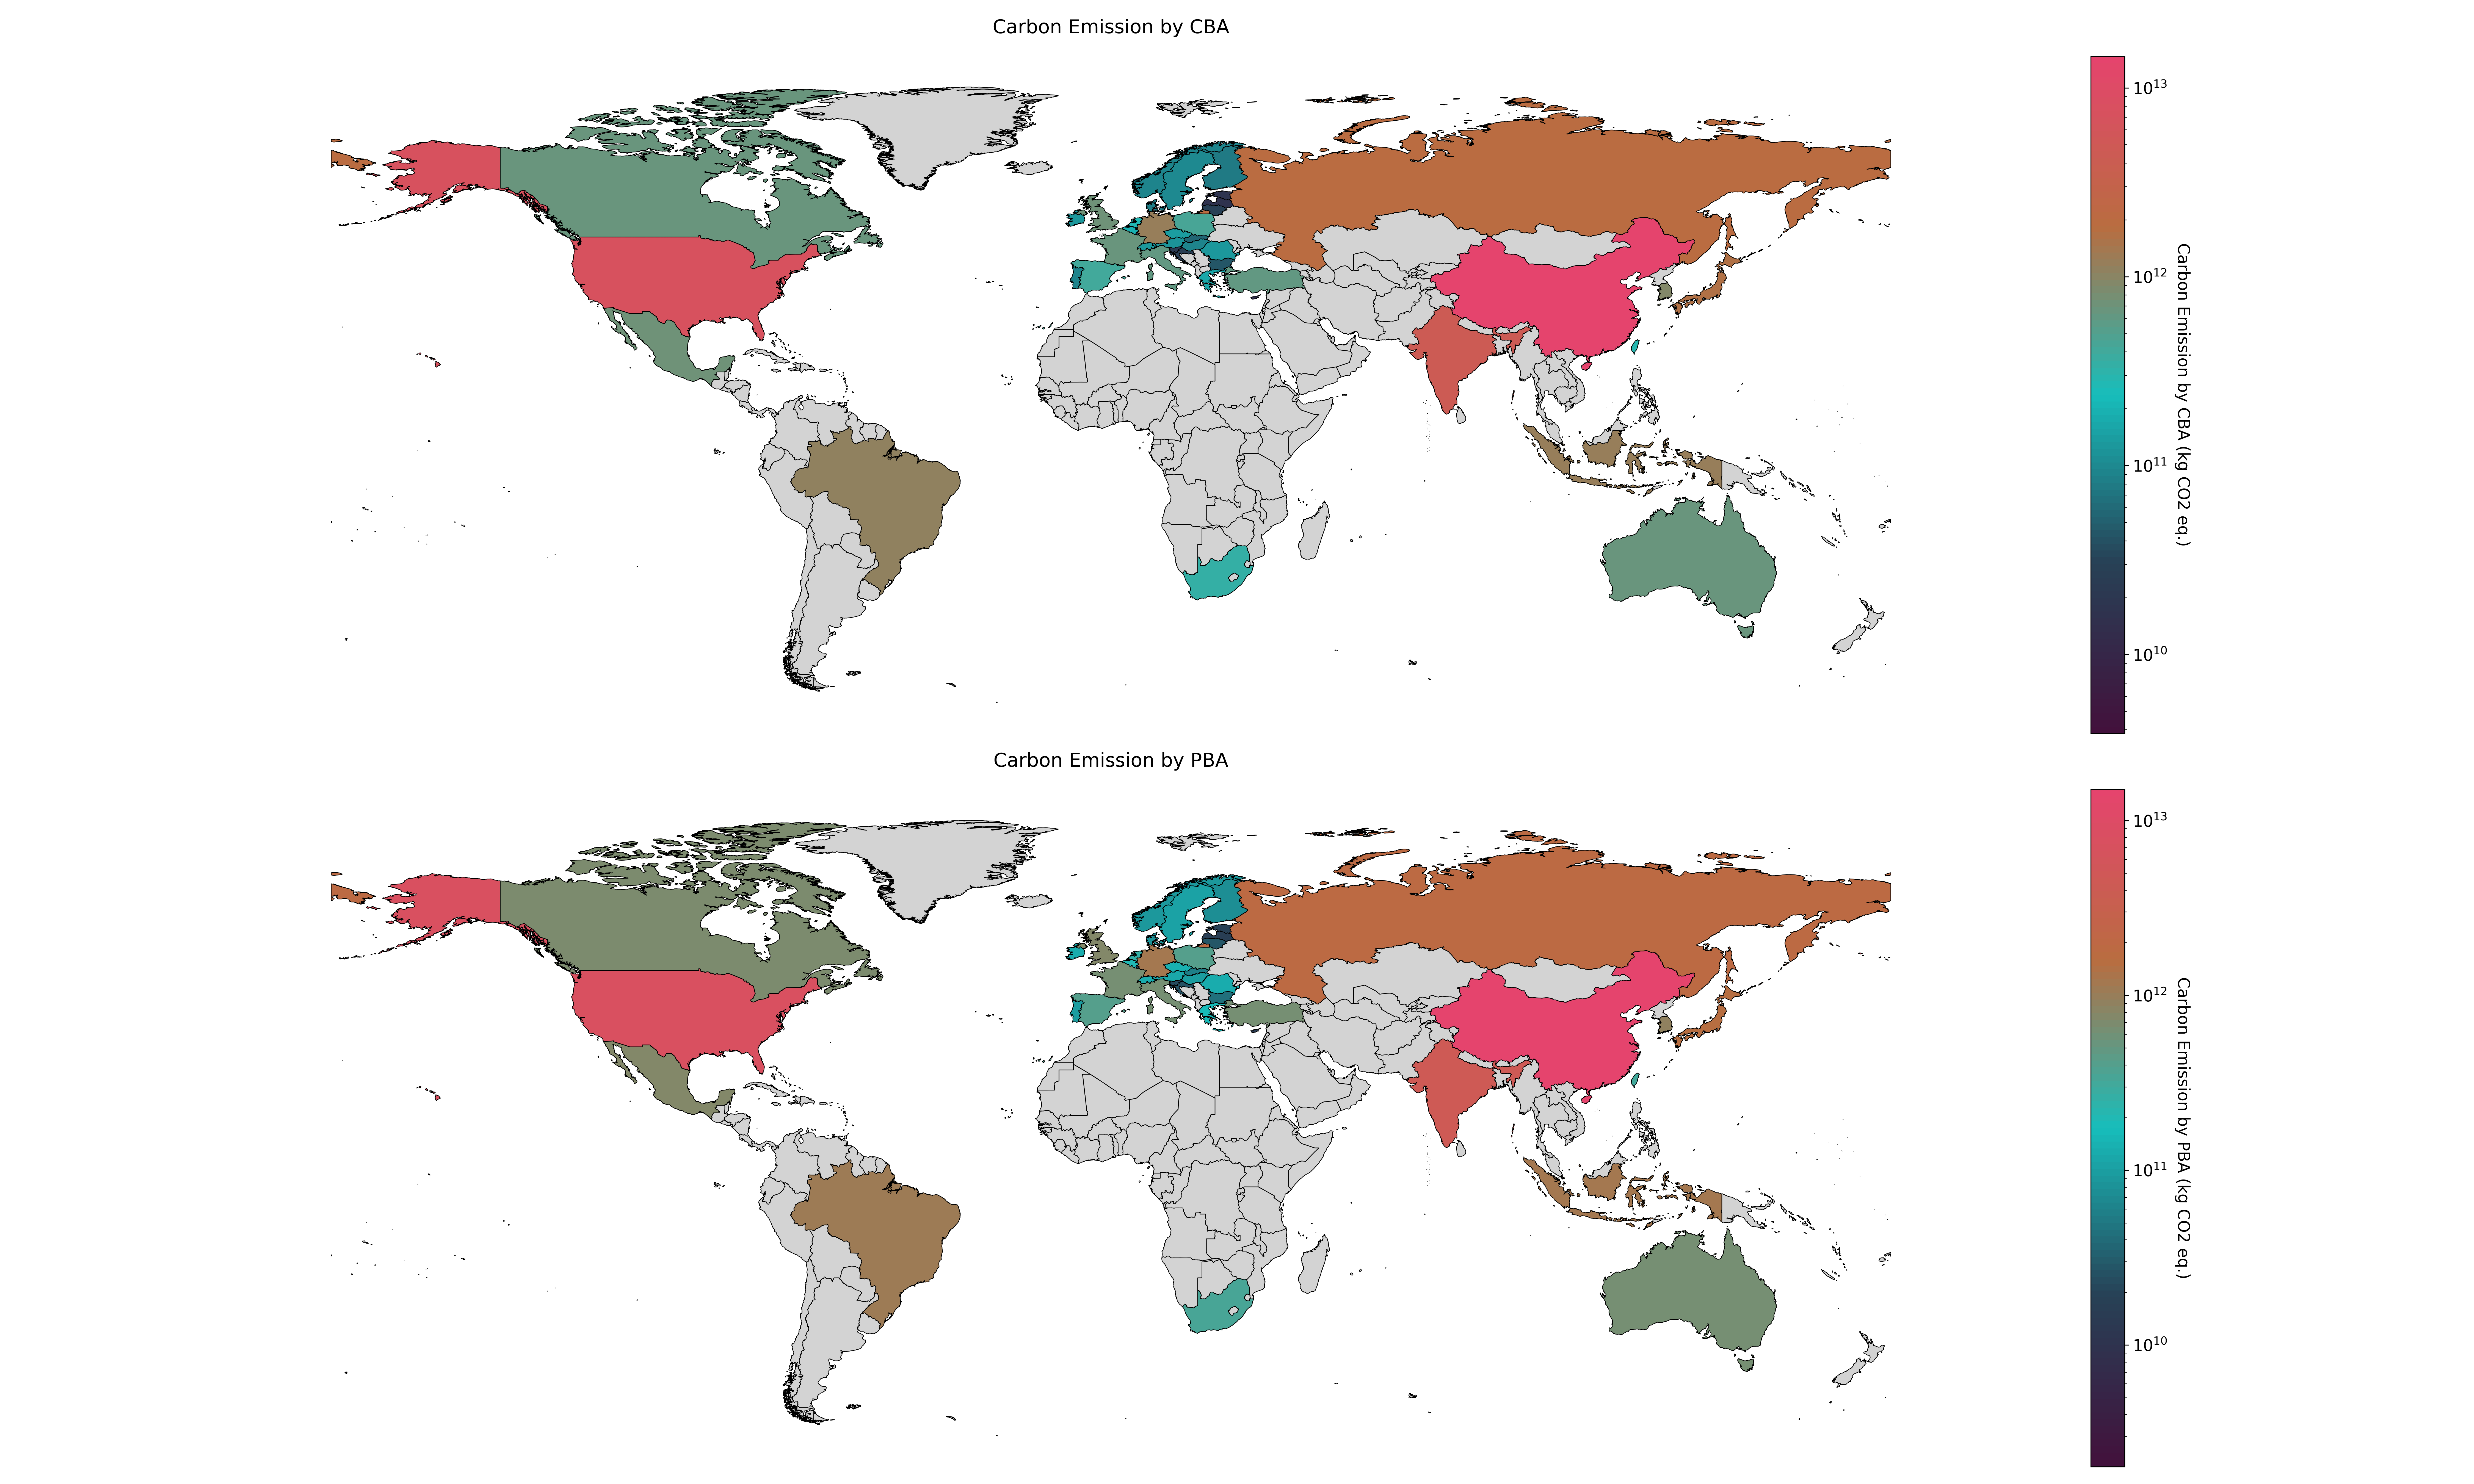
\includegraphics[width=\linewidth]{figures/Graph/Comparison of Carbon Emission (GHG) between PBA and CBA.png}
 \caption{Comparison of Carbon Emission (GHG) between PBA and CBA}\label{fig:Comparison of Carbon Emission (GHG) between PBA and CBA}
\end{sidewaysfigure}
\fi

\subsection{Carbon Uplift in No Trade Scenario}
In the projected scenario where international trade within the semiconductor industry is completely halted, and nations are required to domestically produce what they formerly imported, the data reveal a nuanced tapegraph of carbon uplift percentages across the globe. Figure \ref{fig:Comparison of Carbon Emission (GHG) by CBA and Carbon Uplift} illustrates a marked increase in emissions for several countries. For example, a nation like Germany shows an uplift of 0.26\%, reflecting its high dependency on semiconductor imports and the significant carbon footprint that domestic production would necessitate. Similarly, South Korea, a major player in semiconductor manufacturing, exhibits a 0.19\% increase, which could be attributed to the energy-intensive processes involved in semiconductor fabrication.

On the other end of the spectrum, countries like Saudi Arabia and Russia demonstrate a decrease in carbon emissions, by 0.22\% and 0.35\%, respectively. This surprising trend suggests a possible current overcapacity or a more carbon-efficient domestic production that could replace imports with lower emissions.

Furthermore, the United States, which occupies a central position in the global semiconductor supply chain, shows a potential uplift of 0.29\%, a significant figure given the scale of the country's economy. Meanwhile, China, with its extensive manufacturing infrastructure, sees an uplift of 0.12\%. This lower relative increase may be indicative of its already substantial domestic production capabilities.

The data also bring to light the variable effects on smaller economies such as those in Southeast Asia, where the percentage change swings widely, from a decrease of 0.18\% in countries like Singapore to an increase of 0.31\% in others like Vietnam. These variations emphasize the differing levels of reliance on the global trade of semiconductors and the disparity in carbon emission changes that would result from a shift to self-sufficiency.

This portrayal of carbon uplift, drawn from the dataset, provides a detailed account of the anticipated repercussions on global carbon emissions in the absence of semiconductor trade. It underscores the extent to which international commerce is interwoven with environmental impacts and highlights the potential increase in global carbon footprint that could follow from a turn towards national production in the semiconductor industry.
\ifincludefigures
\begin{sidewaysfigure}
  \centering
  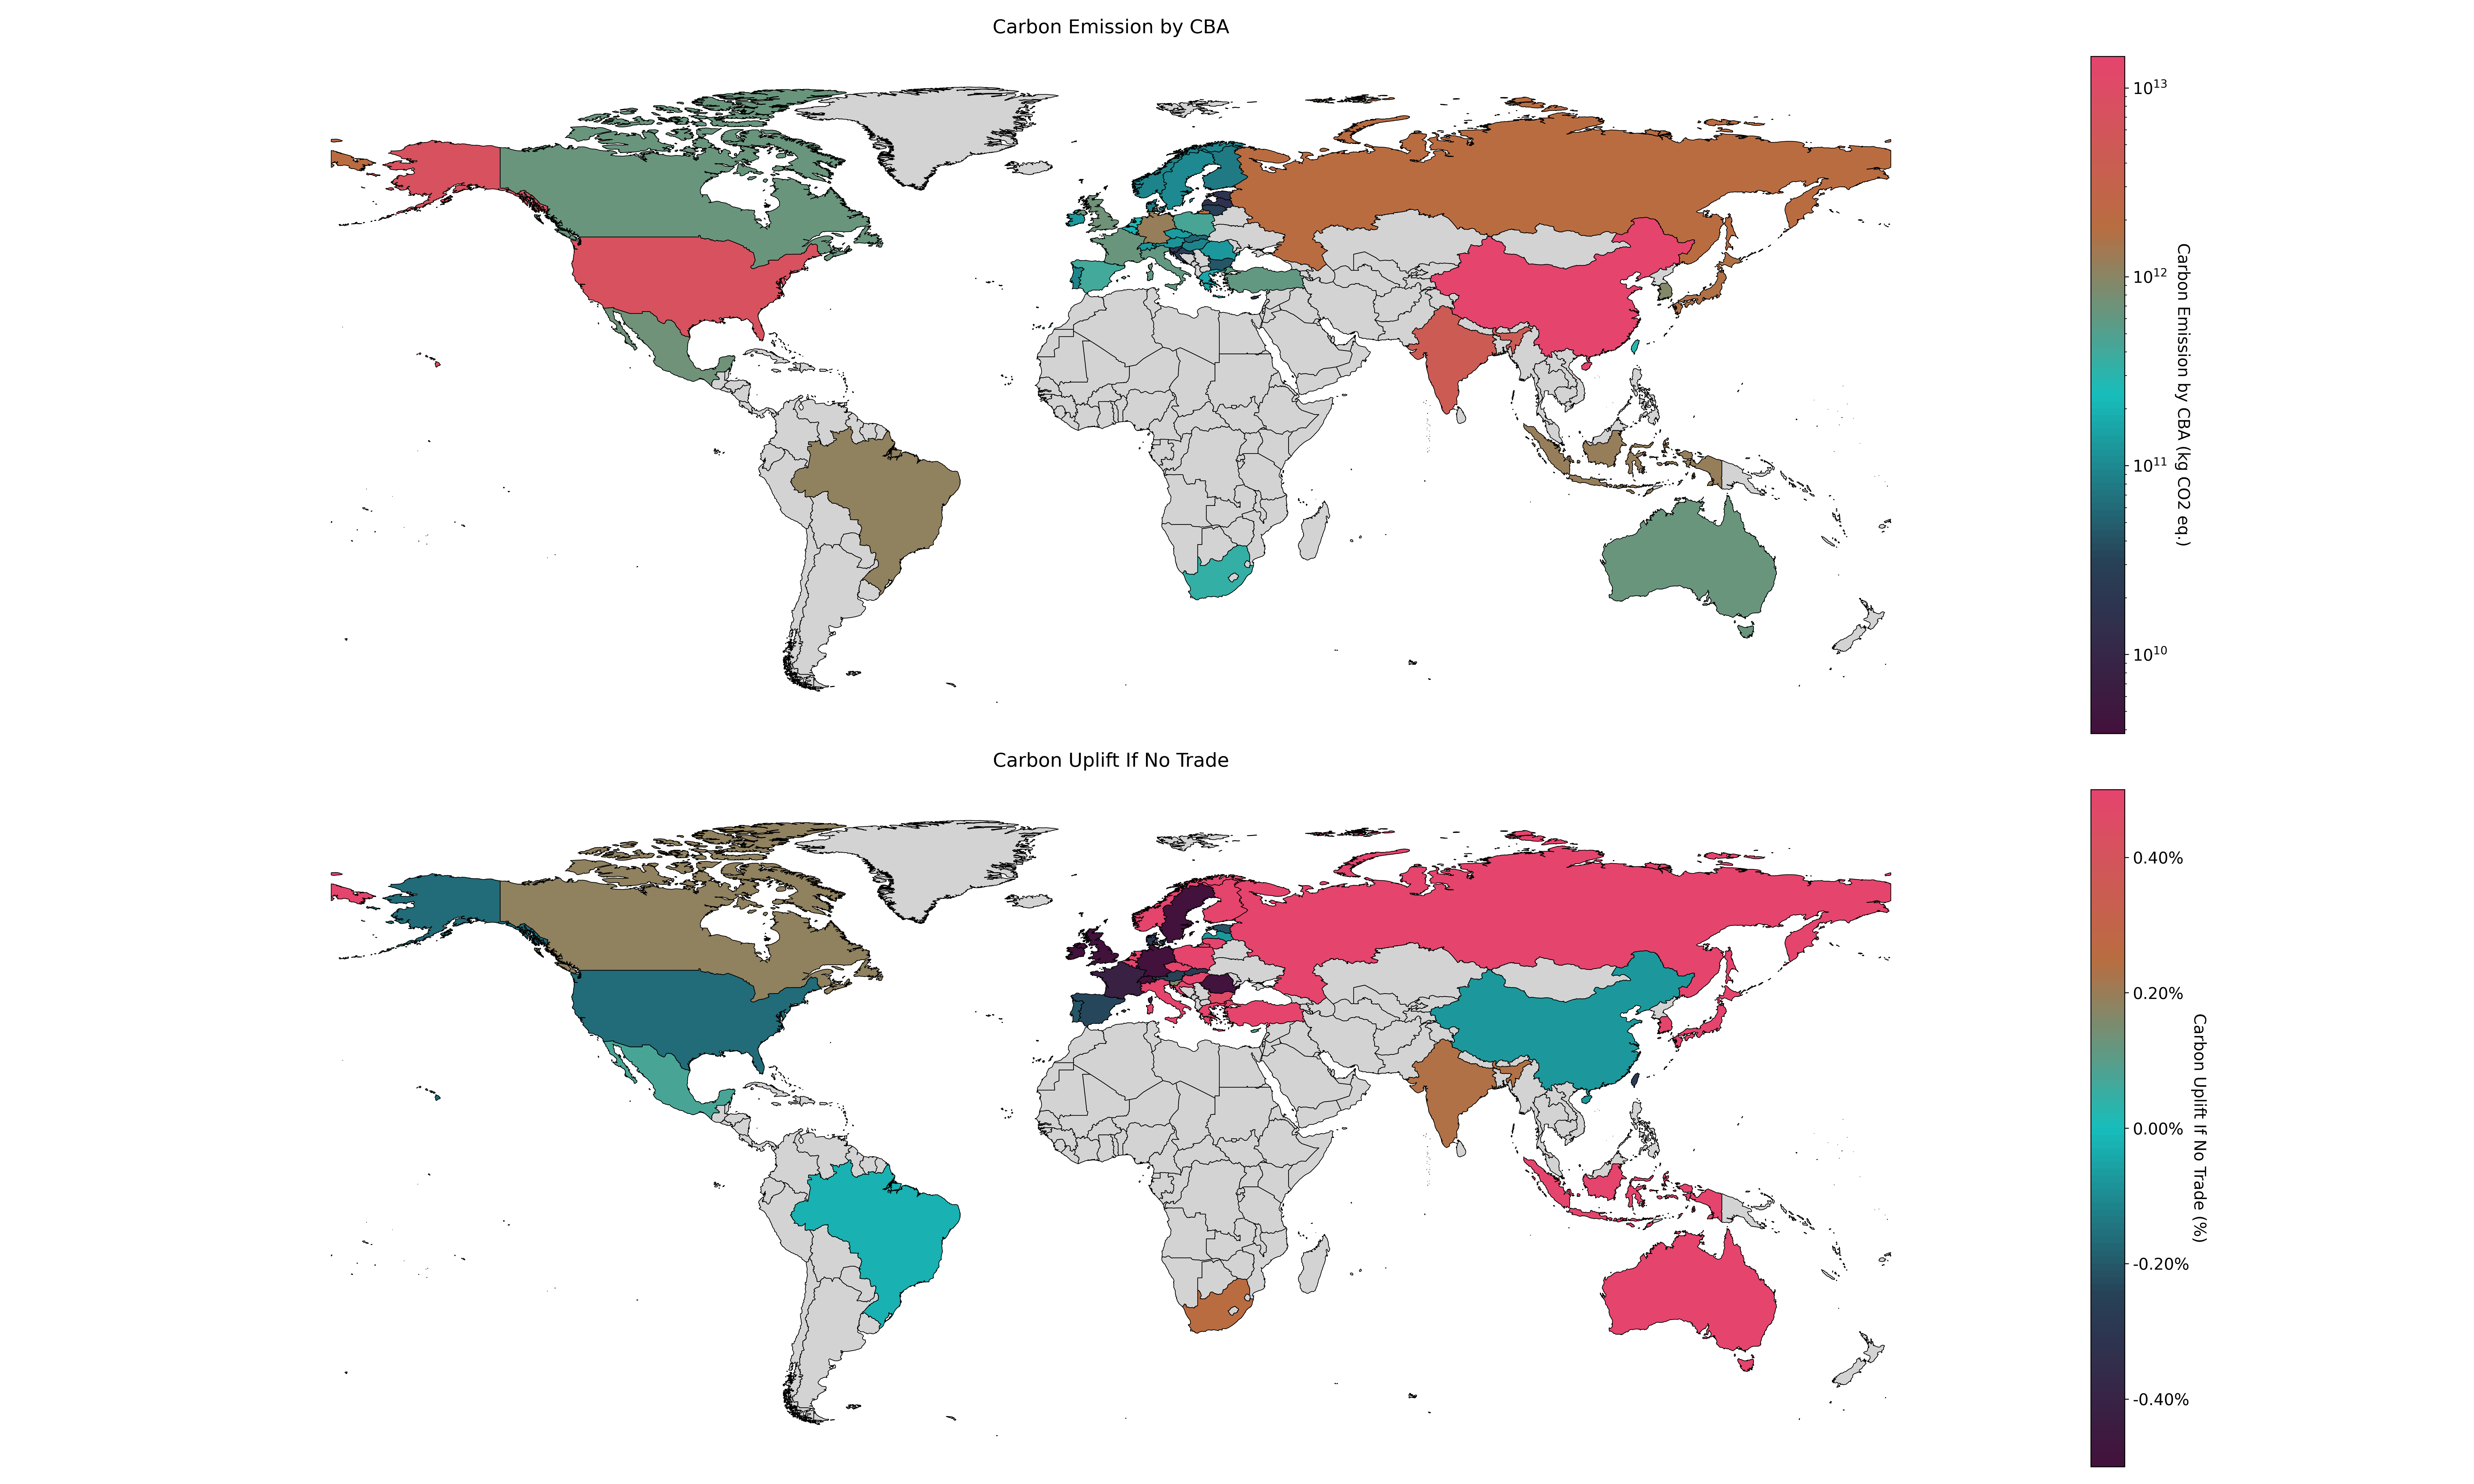
\includegraphics[width=\linewidth]{figures/Graph/Comparison of Carbon Emission (GHG) by CBA and Carbon Uplift.png}
 \caption{Comparison of  Carbon Emission (GHG) by CBA and Carbon Uplift}\label{fig:Comparison of  Carbon Emission (GHG) by CBA and Carbon Uplift}
\end{sidewaysfigure}
\fi

In the compendium of these findings, Figure \ref{fig:Value of Carbon Uplift If No Trade Heatmap in 2022} manifests the hypothetical variance in carbon emissions contingent upon the cessation of trade, particularly within the semiconductor industry's supply chain. The sectors scrutinized are dissected into two principal echelons—upstream and downstream—each critical to the lifecycle of semiconductor production.

In the upstream ambit, the data convey that for ``Other non-ferrous metal ores and concentrates'' China's carbon uplift is approximately -0.053\%, a fractional decrement. The United States records a similar downtrend at -0.045\%. For 'secondary other non-ferrous metals for treatment" both nations effectively exhibit no change, as indicated by the negligible uplift values close to zero.

The downstream analysis for ``Electrical machinery and apparatus n.e.c. (31)'' and ``Office machinery and computers (30)'' denotes a -0.023\% and -0.006\% carbon uplift for China, respectively. The United States reflects a more pronounced -0.050\% reduction in the ``Electrical machinery'' sector and a slight increase of 0.004\% in the ``Office machinery'' sector. The slight increase for the U.S. in the ``Office machinery'' sector diverges from the overall downward trend observed in other sectors.

``Radio, television and communication equipment and apparatus (32)'' sees an uplift of approximately 0.003\% for China, contrasting with a -0.030\% reduction for the United States. For ``Medical, precision and optical instruments, watches and clocks (33)'' China's figures suggest a -0.023\% decrease, while the United States presents a -0.033\% reduction.

When evaluating the aggregated data for all semiconductor-related products, China showcases a carbon uplift of -0.077\% across related products, -0.028\% for upstream, and -0.049\% for downstream products. The United States, however, reveals a more substantial decrease across these categories, with -0.168\% for related products, -0.059\% for upstream, and -0.109\% for downstream sectors.

These percentages suggest that in the hypothetical scenario of a no-trade environment, both China and the United States would experience a decrease in carbon emissions across most semiconductor sectors, with the United States displaying a marginally greater reduction. This trend aligns with the broader global efforts to achieve carbon neutrality, yet it underscores the criticality of trade in optimizing the carbon efficiency of the semiconductor supply chain.

Conversely, many other countries may rely heavily on the import of semiconductors and related products, lacking the same level of infrastructure or technological prowess. If these nations were compelled to produce semiconductors domestically, they might need to invest in new facilities and processes, which could be less efficient and more carbon-intensive than those available in countries like China and the United States. Additionally, the scale of production could affect emissions; smaller-scale operations may not benefit from the same efficiencies as larger ones.

Moreover, the overall increase in global carbon emissions reflects the intricate and optimized nature of the current global trade network. Specialized production and economies of scale in certain regions lead to a reduced carbon footprint per unit of output. When this specialization is absent, as in a no-trade scenario, production may become less efficient globally, leading to higher carbon emissions.

This interplay of regional specialization, technological disparities, and economies of scale forms the crux of the potential increase in global carbon emissions in the absence of trade. The heatmap, while highlighting the outliers in China and the United States, simultaneously reveals that the global picture is one of increased carbon output, underlying the critical role of trade in not only economic efficiency but also in the pursuit of environmental sustainability.
\ifincludefigures
\begin{figure}
 \centering
 \makebox[\textwidth][c]{\includegraphics[width=1\textwidth]{figures/Graph/Value of Carbon Uplift If No Trade Heatmap in 2022.png}}
 \caption{Value of Carbon Uplift If No Trade Heat Map in 2022}\label{fig:Value of Carbon Uplift If No Trade Heatmap in 2022}
\end{figure}
\fi

\subsection{Carbon Uplift in No Sino-US Trade Scenario}

In the examination of the projected carbon uplift in the hypothetical scenario of no trade between China and the United States, we unveil distinct patterns within the semiconductor industry's upstream and downstream sectors. This analysis is predicated on the percentage change in carbon emissions, encapsulated within the data points provided.

For the upstream sector, ``Other non-ferrous metal ores and concentrates'' the data reflects a negligible decrease in emissions for China at approximately -0.0001\%, and an increase for the United States at approximately 0.0047\%. In the adjacent sector of 'secondary other non-ferrous metals for treatment" both nations appear to maintain an invariant emission level, suggested by the uplift values insignificantly close to zero.

Within the realm of precious metals, China's emissions present a slight increase of 0.0041\%, while the United States exhibits a more significant decrease of -0.0101\%. The data for ``secondary precious metals for treatment'' remains effectively unchanged for both countries, akin to the pattern observed in the 'secondary other non-ferrous metals for treatment" sector.

Delving into the downstream sectors, ``Electrical machinery and apparatus n.e.c. (31)'' for China shows a reduction in emissions by -0.0005\%, contrasted by an increase of 0.0093\% for the United States. For ``Office machinery and computers (30)'' China's carbon uplift is -0.0003\%, whereas the United States sees an augmentation by 0.0172\%. ``Radio, television and communication equipment and apparatus (32)'' records a decrease for both countries, with China at -0.0002\% and the United States at -0.0053\%. The sector of ``Medical, precision and optical instruments, watches and clocks (33)'' exhibits a decrease in emissions for China by -0.0023\ and an increase for the United States by 0.0054\%.

Aggregating the sectors under ``semiconductivity Related Products'' China demonstrates a slight increase of 0.0114\%, while the United States shows a notable increase of 0.0212\%. In ``semiconductivity Upstream Products'' both countries experience an increase, with China at 0.0041\% and the United States at -0.0054\%. For 'semiconductivity Downstream Products" China shows a decrease of -0.0029\%, and the United States a more significant increase of 0.0266\%.

The variegated data implicates that in the absence of bilateral trade, both China and the United States would experience a mix of increases and decreases in carbon emissions across different sectors. The United States, in particular, shows larger percentage changes both in terms of decreases and increases. This disparity likely stems from the comparative advantage inherent within each nation's industrial complex, emphasizing the nuanced interdependence between the two superpowers within the global semiconductor market.

It is this delicate equilibrium of trade, production efficiencies, and carbon emissions that Figure \ref{fig:Value of Carbon Uplift If No Sino-US Trade Heatmap in 2022} strives to visually articulate. The color-coded cells, each corresponding to a unique data point, reveal a tapestry of potential outcomes that are instrumental in contextualizing the environmental implications of trade policies within the semiconductor industry.
\ifincludefigures 
\begin{figure}
 \centering
 \makebox[\textwidth][c]{\includegraphics[width=1\textwidth]{figures/Graph/Value of Carbon Uplift If No Sino-US Trade Heatmap in 2022.png}}
 \caption{Value of Carbon Uplift If No Sino-US Trade Heat Map in 2022}\label{fig:Value of Carbon Uplift If No Sino-US Trade Heatmap in 2022}
\end{figure}
\fi
\subsection{Carbon Uplift in No Sino-US with Gaming Trade Scenario}

Figure \ref{fig:Value of Carbon Uplift If No Sino-US with Gaming Trade Heatmap in 2022} provided delineates the carbon uplift, articulated as a direct consequence of a trade rearrangement modeled on game-theoretic principles for the year 2022. This analysis illuminates the carbon footprint repercussions in various industrial sectors, with a spotlight on semiconductivity.

For China, the data indicates a notable carbon uplift of 1.2301\% in the semiconductivity related products sector. This represents a significant environmental benefit accruing from the hypothetical trade reallocation. Conversely, there is a marginal contraction of -0.0148\% in the semiconductivity upstream products, counterbalanced by an uplift of 0.3482\% in the downstream products.

The United States displays a more modest uplift of 0.0773\% in semiconductivity related products, suggesting a lesser but still positive environmental impact from the trade redistribution. A negligible decrease of -0.0013\% is observed in the upstream products, while downstream products experience an uplift of 0.1903\%.

Globally, the analysis reflects a carbon uplift of 0.3568\% in semiconductivity related products, with a slight decrease of -0.0043\% in the upstream sector. The downstream sector sees an uplift of 0.1229\%, underscoring the significant environmental impacts within the semiconductor supply chain on a global scale.

Such data exemplifies the critical role of trade patterns in shaping carbon emission trajectories. It reveals that strategic trade reallocations can potentially lead to an enhancement or deterioration of environmental outcomes, particularly within high-tech and high-impact sectors like semiconductivity.

This granular perspective allows us to infer not only the environmental implications of these strategic decisions but also the differential impacts that such redistributions might engender across various production stages. It emphasizes the need for an integrated approach to trade policy, one that takes into account the complex interdependencies within global supply chains and their environmental ramifications.
\ifincludefigures
\begin{figure}
  \centering
  \makebox[\textwidth][c]{\includegraphics[width=1\textwidth]{figures/Graph/Value of Carbon Uplift If No Sino-US with Gaming Trade Heatmap in 2022.png}}
  \caption{Value of Carbon Uplift If No Sino-US with Gaming Trade Heatmap in 2022}\label{fig:Value of Carbon Uplift If No Sino-US with Gaming Trade Heatmap in 2022}
 \end{figure}
\fi
\section{How does Semi-conductor Related Products Trade Impact Global Carbon Emissions}

\subsection{Carbon Uplift in No Semi-conductor Related Products Trade Scenario}

Figure \ref{fig:Carbon Uplift If No Trade 2022} displays the percentage change in carbon emissions in the scenario of no semiconductor trade, segregated into three categories: related products, upstream products, and downstream products.

The global percentage change in carbon emissions for semiconductivity related products shows an increase, indicating that on a worldwide scale, ceasing trade in this category would lead to an uptick in emissions due to domestic production.

However, some countries like the United States and China exhibit a decrease in carbon emissions across all three sectors. This could suggest that these countries are currently producing these goods more efficiently than the global average, and shifting to domestic production exclusively might actually decrease their carbon emissions in these categories.

For example, the United States shows a decrease of 0.2495\% in related products, a decrease of 0.1300\% in upstream products, and a decrease of 0.1195\% in downstream products. Similarly, China's data indicates a decrease of 0.2070\% in upstream products and a 0.0184\% decrease in downstream products, which may reflect the high efficiency and scale of their existing semiconductor manufacturing capabilities.

On the other hand, for countries where an increase is observed, such as those that might be more import-reliant for these products, the need to develop or expand domestic production may lead to higher emissions compared to the current state of trade.

The specific increases or decreases in the respective sectors for each country will guide us in understanding the potential environmental impact of shifts in the semiconductor trade policy and production landscape. It is important to note that these figures are subject to the nuances of each country's existing industrial capabilities and the complexity of the semiconductor supply chain. 
\ifincludefigures 
\begin{figure}
 \centering
 \makebox[\textwidth][c]{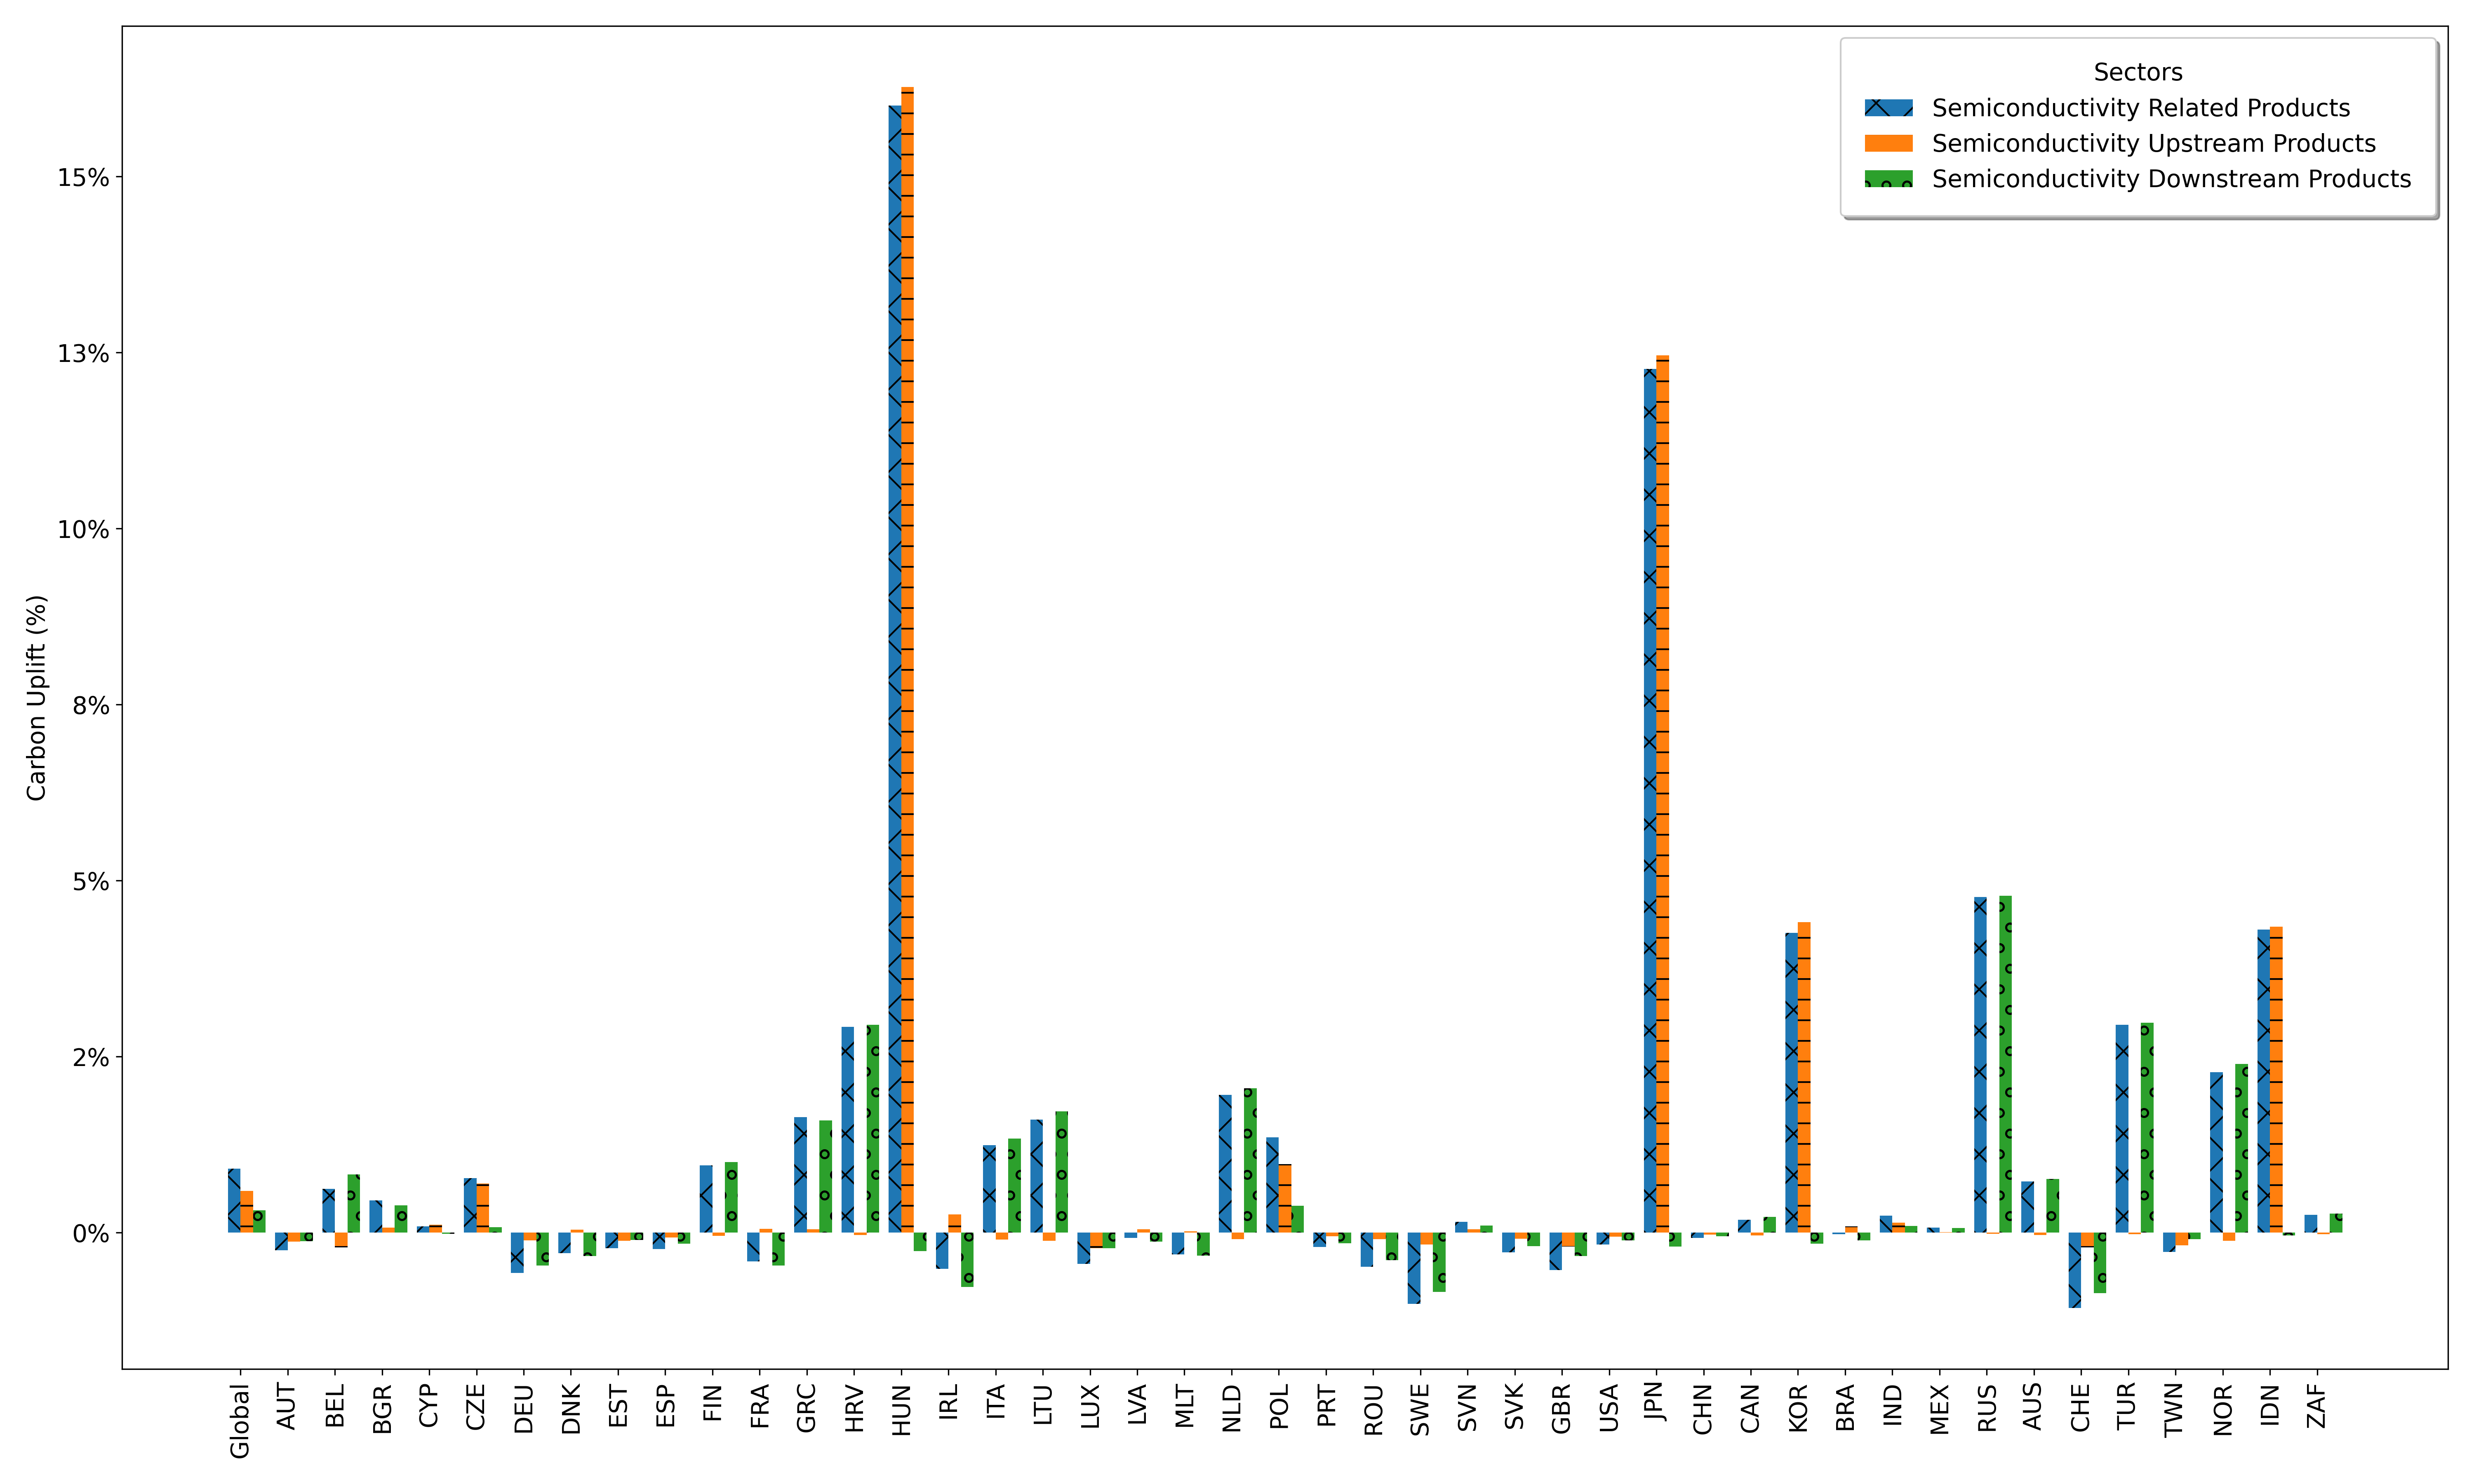
\includegraphics[width=1\textwidth]{figures/Graph/Carbon Uplift If No Trade 2022.png}}
 \caption{Carbon Uplift If No Trade 2022}\label{fig:Carbon Uplift If No Trade 2022}
\end{figure}
\fi
Figure \ref{fig:Carbon Uplift Trends If No Trade(2000-2022)} meticulously plots the trajectory of carbon emission changes under a theoretical framework where no trade exists. Focusing on the semiconductor industry, the data is bifurcated into related, upstream, and downstream products over a span of two decades, encapsulating the temporal evolution of carbon uplift percentages for both China (CN) and the United States of America (US).

From the dawn of the millennium in 2000, we observe China's carbon uplift in semiconductivity related products initiating at approximately 0.0348\%, with a shift towards a reduction in emissions across all sectors by 2022, landing at -0.0768\%. Notably, the trajectory exhibits a downward trend, punctuated by fluctuating increments, particularly evident in the upstream products sector, which sees an initial increase to 0.0257\% in 2000, followed by a decrease to -0.0279\% by 2022. The downstream products sector for China reflects this decrement more modestly, from 0.0091\% in 2000 to -0.0488\% in 2022.

The United States presents a distinct pattern; the carbon uplift in semiconductivity related products starts at -0.0425\% in 2000 and deepens to -0.1678\% by 2022. This significant downward trajectory suggests an increasing efficiency in carbon emissions over time. The upstream sector undergoes a remarkable decrease from -0.0244\% in 2000 to -0.0590\% in 2022, emphasizing a consistent focus on reducing carbon intensity. The downstream sector echoes this trend, commencing at -0.0181\% in 2000 and culminating at -0.1088\% in 2022, underscoring the role of technological advancements and efficiency improvements.

In the broader global context, the carbon uplift exhibits an overall escalation, suggesting that while individual nations such as China and the United States may optimize and reduce their carbon footprint, the aggregate global emissions could potentially rise in the absence of international trade. This scenario accentuates the integral role of global trade mechanisms in distributing the production of semiconductors to locations where carbon efficiency is maximized.

The data, set against the backdrop of the intricate interactions of the semiconductor industry's global supply chain, serves as an empirical testament to the environmental implications of trade policies and the technological evolutions within this pivotal sector. As the author of this analysis, the intent is not only to present these data points but also to foster a dialogue on the role of international cooperation in mitigating carbon emissions, underpinning the necessity of a symbiotic approach to trade and environmental sustainability.
\ifincludefigures
\begin{figure}
\centering
\makebox[\textwidth][c]{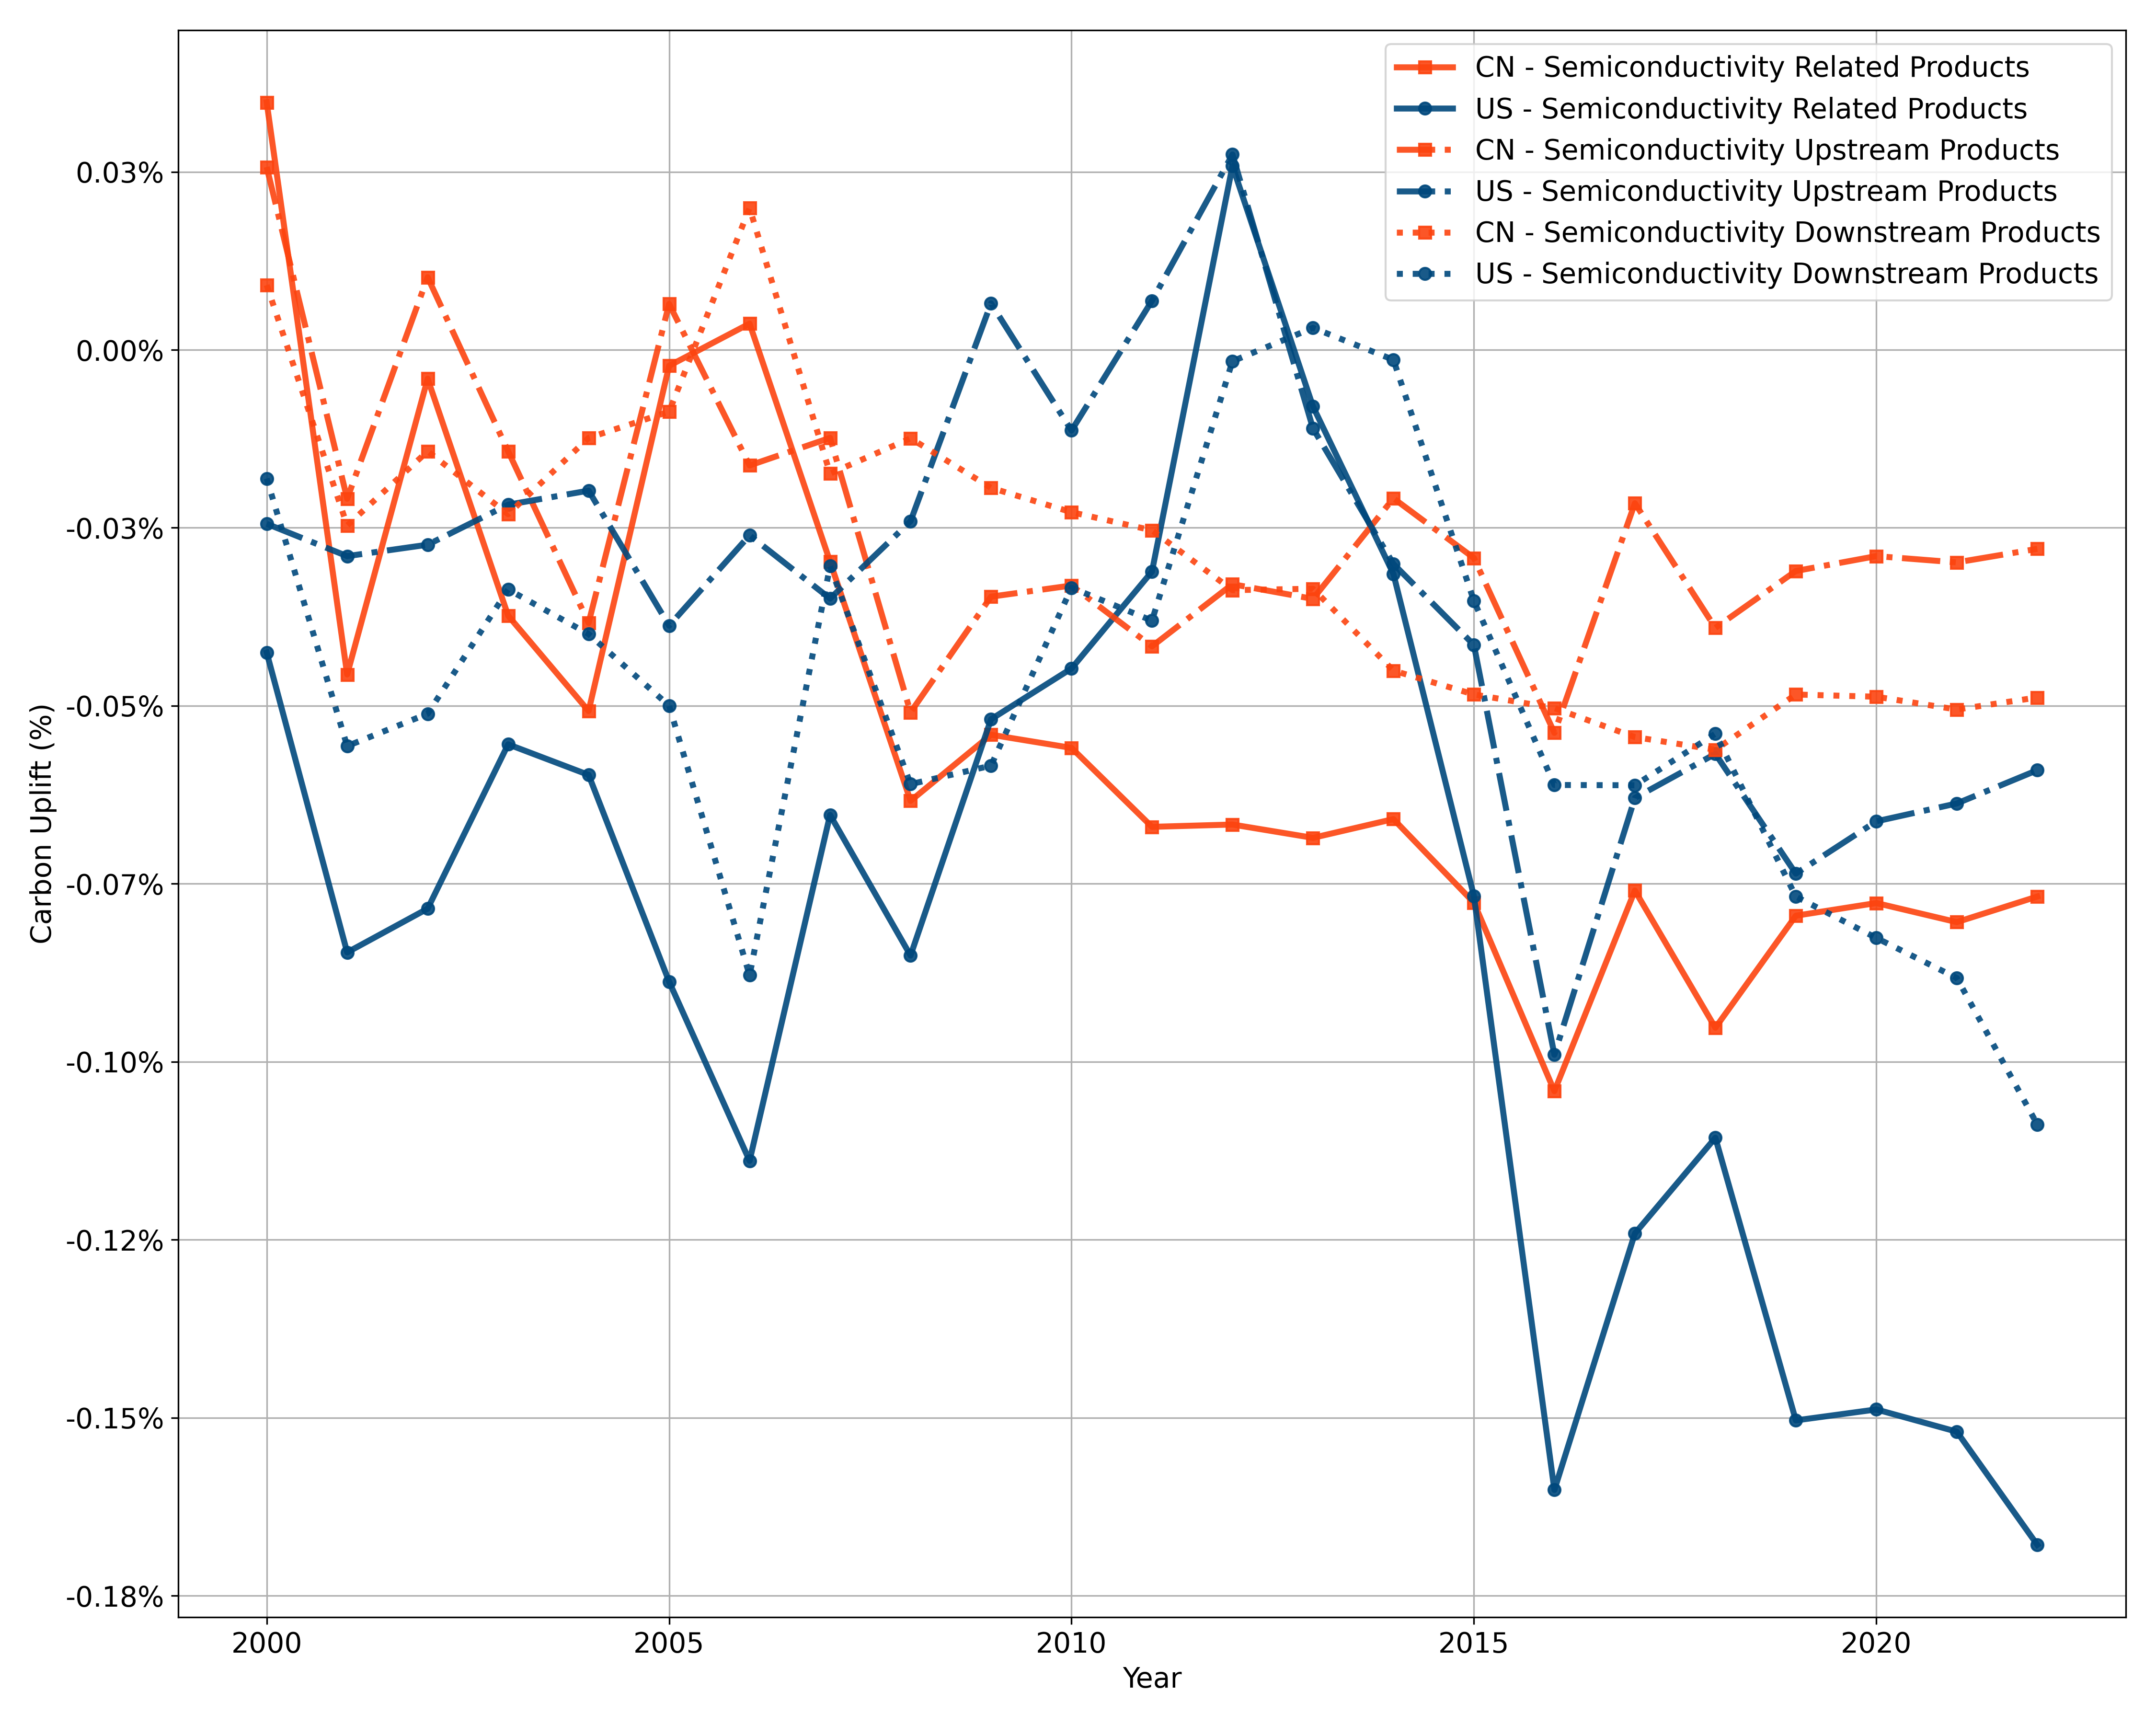
\includegraphics[width=1\textwidth]{figures/Graph/Carbon Uplift Trends If No Trade(2000-2022).png}}
\caption{Carbon Uplift Trends If No Trade(2000-2022)}\label{fig:Carbon Uplift Trends If No Trade(2000-2022)}
\end{figure}
\fi
\subsection{Carbon Uplift in No Sino-US Semi-conductor Related Products Trade Scenario}


The comparative analysis of carbon emission uplift under no trade scenarios, globally and between China and the United States, Figure \ref{fig:Comparison of Carbon Uplift between No Trade Scenario and No Sino-US Trade Scenario} provides pivotal insights into the environmental repercussions of trade policies. In a no-trade environment, the assumption is that previously imported goods are entirely substituted by domestic production, leading to an increase in carbon emissions due to the shift in production dynamics.

Globally, the absence of trade would result in a carbon uplift of 0.9106\% for semiconductivity-related products, 0.5956\% for upstream products, and 0.3152\% for downstream products. This indicates a not insignificant surge in emissions, positing that the global market relies on trade to maintain lower carbon output levels through more efficient production distributions.

In contrast, China shows a reduction in carbon uplift across all categories when trade is absent, with -0.0768\% for related products, -0.0280\% for upstream, and -0.0488\% for downstream sectors. This can be interpreted as China's industrial sector possibly benefiting from the import of less carbon-intensive goods, or indicating a high efficiency in certain domestic productions that would otherwise be replaced by imports.

The United States presents a different picture, with a substantial carbon uplift reduction when trade is eliminated: -0.1678\% for related products, -0.0590\% for upstream, and -0.1088\% for downstream sectors. This suggests that the U.S. may be offloading more carbon-intensive production to trade partners and would see an environmental benefit in terms of carbon emissions if it were to produce these goods domestically.

When examining the scenario where only Sino-U.S. trade is halted, we observe a minimal global carbon uplift of 0.0031\% for related products, 0.0004\% for upstream, and 0.0026\% for downstream products. This negligible change suggests that while the Sino-U.S. trade relationship is significant, other global trade activities maintain the predominant share of carbon emission contributions.

China's carbon uplift in a no Sino-U.S. trade scenario slightly increases for semiconductivity-related and upstream products, with 0.0011\% and 0.0041\% respectively, yet the downstream sector shows a reduction, reflecting the nuanced impacts across different sectors. For the United States, the absence of bilateral trade with China reveals a carbon uplift of 0.0212\% for related products and a notable increase for downstream products by 0.0266\%, again underscoring the complexity of sector-specific trade impacts on carbon emissions.
\ifincludefigures 
\begin{figure}
 \centering
 \makebox[\textwidth][c]{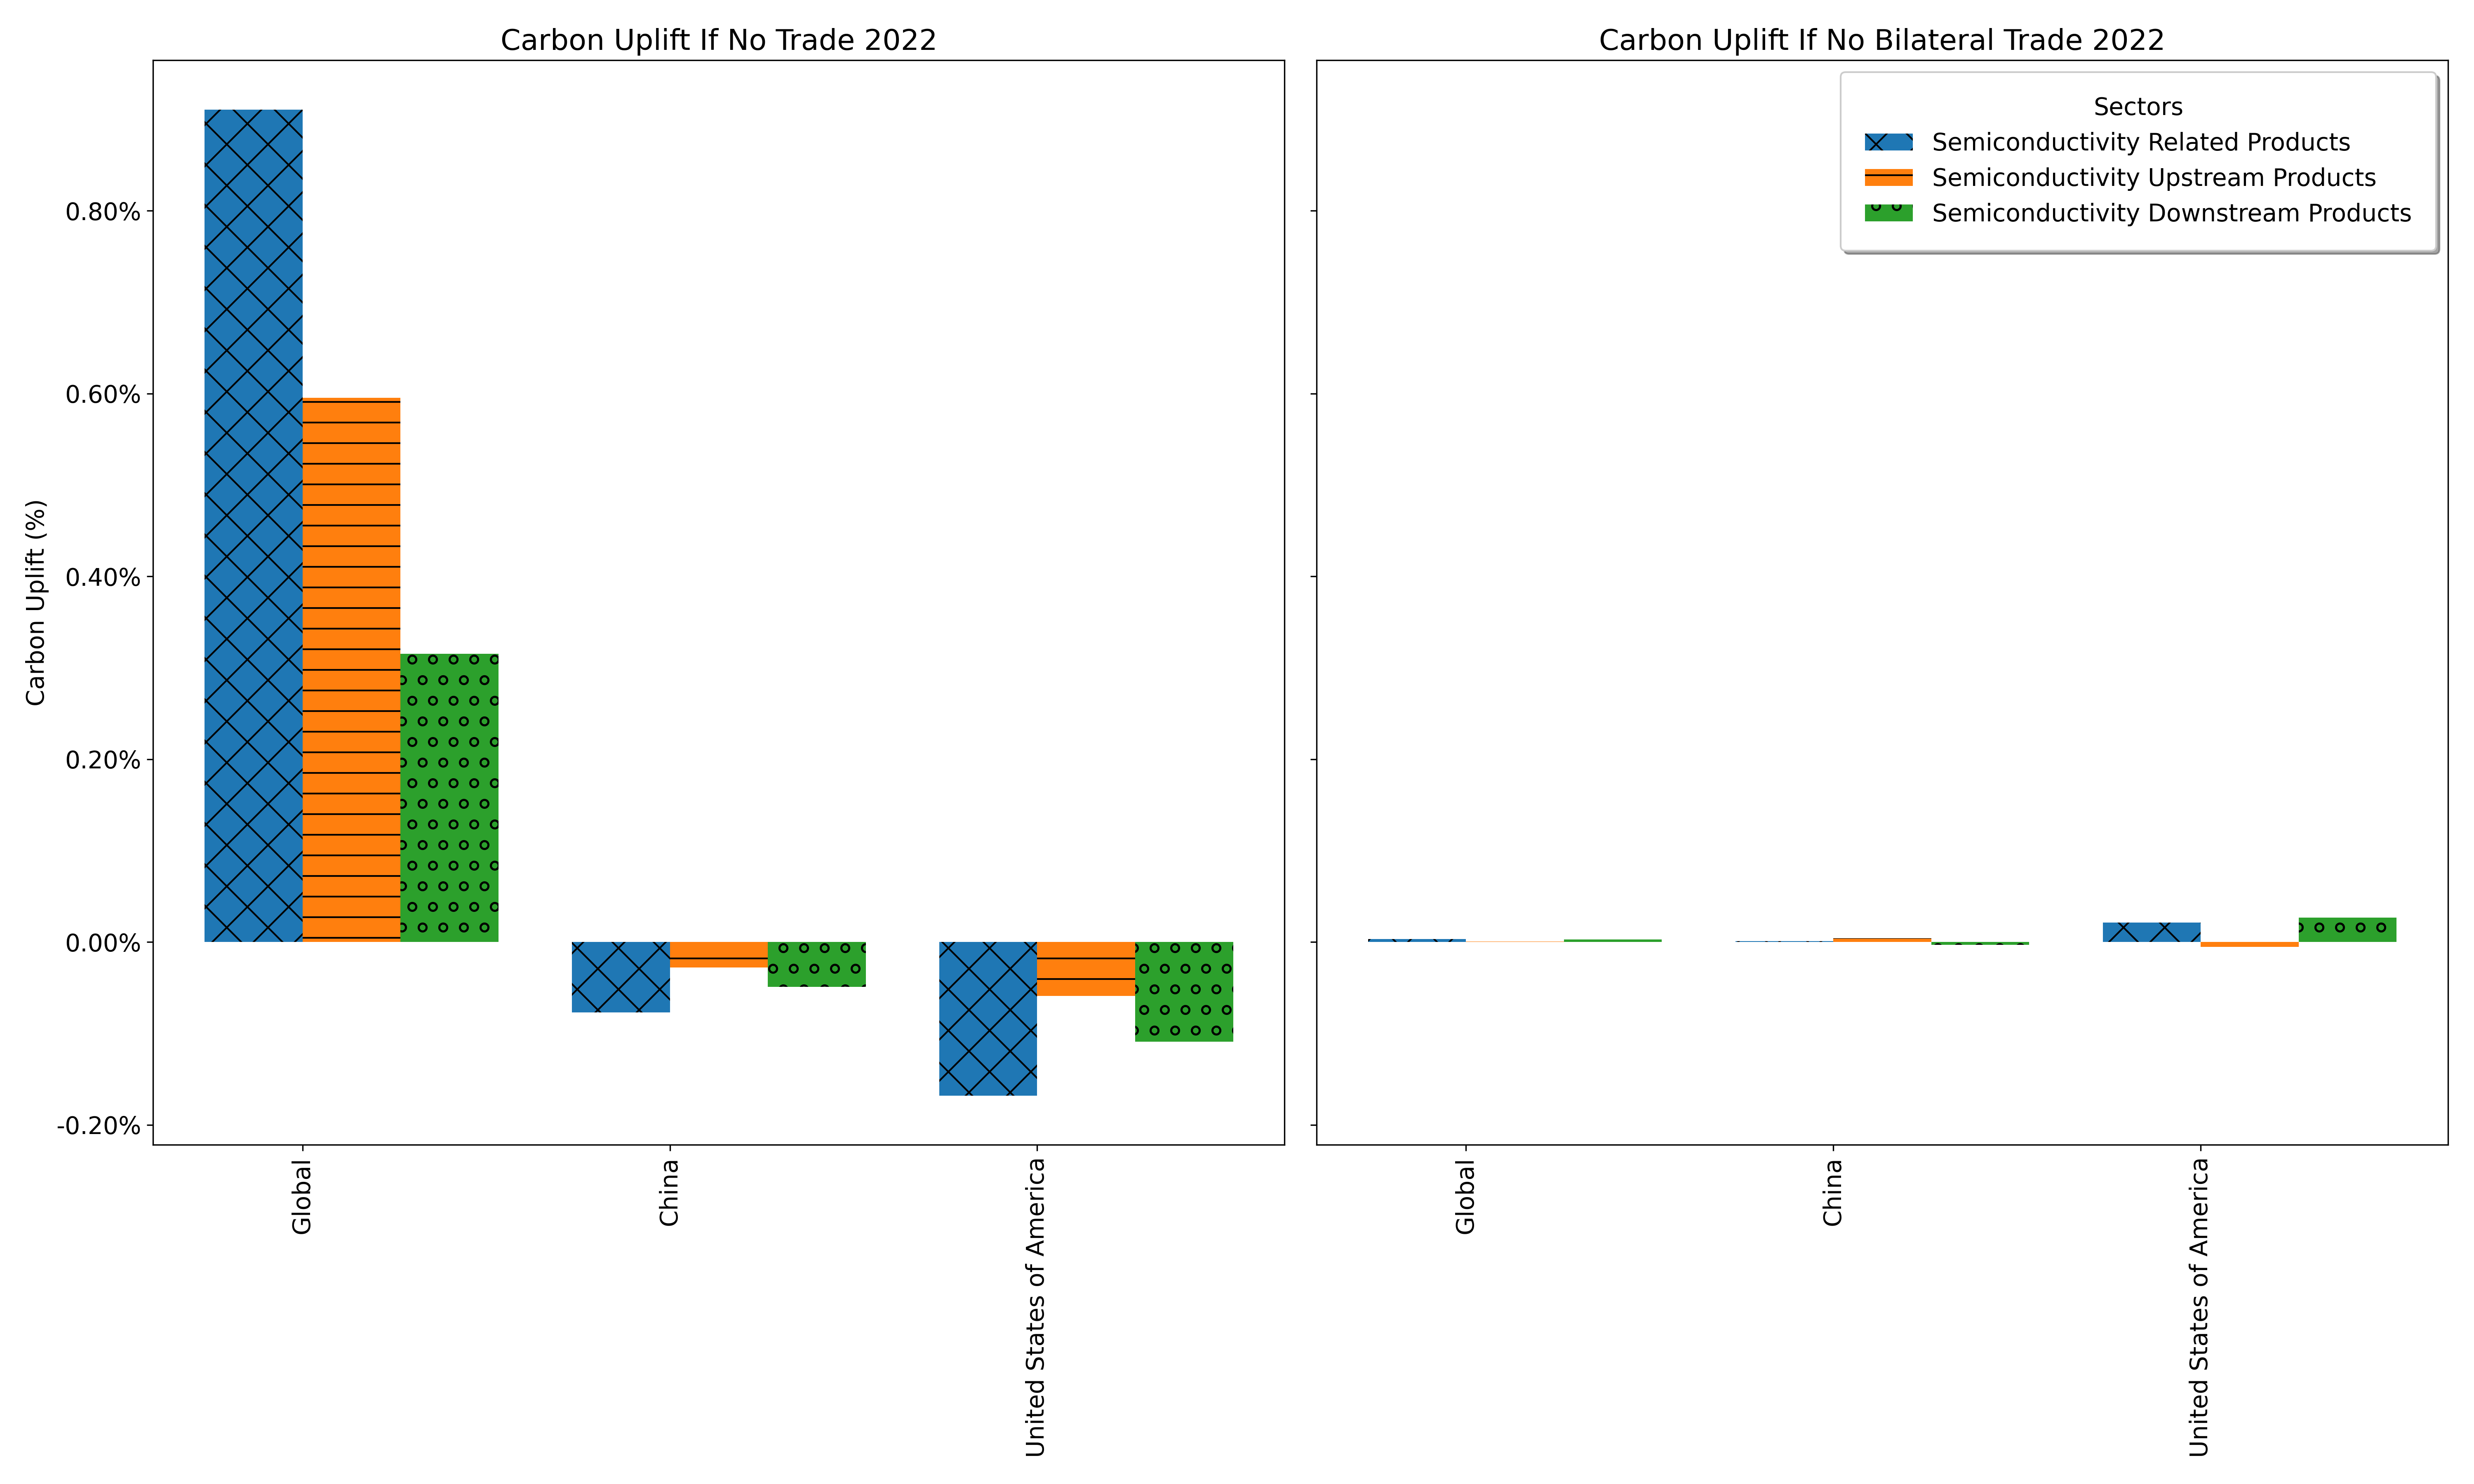
\includegraphics[width=1\textwidth]{figures/Graph/Comparison of Carbon Uplift between No Trade Scenario and No Sino-US Trade Scenario.png}}
 \caption{Comparison of Carbon Uplift between No Trade Scenario and No Sino-US Trade Scenario}\label{fig:Comparison of Carbon Uplift between No Trade Scenario and No Sino-US Trade Scenario}
\end{figure}
\fi
In the analysis presented here, the graph Figure \ref{fig:Carbon Uplift Trends If No Sino-US Trade(2000-2022)} reflects the implications of a scenario where the established trade links between China and the United States in the semiconductor industry are disrupted. This graph elucidates the carbon uplift, or the potential increase in carbon emissions due to changes in production dynamics resulting from such a trade cessation.

The data suggests that China's semiconductor industry exhibits a relatively stable carbon uplift throughout the observed period, with minor fluctuations. For instance, in 2000, the carbon uplift in semiconductivity related products was recorded at approximately 0.0047\%, and this figure saw marginal variation, culminating in an uplift of 0.0114\% by 2022. This stability can be attributed to China's mature and comprehensive supply chain, which has developed a certain resilience and capacity for self-sufficiency. Even in the absence of trade with the United States, China's integrated production capabilities enable the maintenance of carbon emissions efficiency, a testament to the robustness of its domestic semiconductor industry.

Conversely, the United States demonstrates a more pronounced variability in carbon uplift. Starting with a carbon uplift reduction in related products of -0.0286\% in 2000, the United States experiences a trend that moves towards an increase of 0.0212\% in 2022. This reflects a significant reliance on Chinese imports within the US semiconductor supply chain. The cessation of trade with China necessitates a shift to internal production, which, despite improvements in carbon emission efficiency over the years, still results in a notable increase in the carbon uplift. Although there is a clear trend of improvement in the United States" carbon efficiency, as evidenced by a gradual decrease in carbon uplift in recent years, the level of uplift remains substantially higher compared to when trade links with China are operational.

The graph offers a visual representation of the divergence in carbon uplift trajectories between the two nations over two decades. The trends indicate that while China has managed to maintain a relatively stable carbon footprint within its semiconductor industry, the United States faces more significant challenges when deprived of its trade partnership with China. Despite advancements in emission reduction techniques, the United States still faces potential increases in carbon emissions in the semiconductor sector in the absence of trade with China.

In conclusion, this data analysis reveals the intricate relationship between international trade and carbon emissions within the semiconductor industry. It underscores the impact of trade policies on environmental sustainability and emphasizes the need for robust supply chains and technological innovation in mitigating carbon emissions. These findings point to the critical importance of international cooperation in achieving a more carbon-efficient global economy, particularly in industries vital to technological progress and development.
\ifincludefigures
\begin{figure}
 \centering
 \makebox[\textwidth][c]{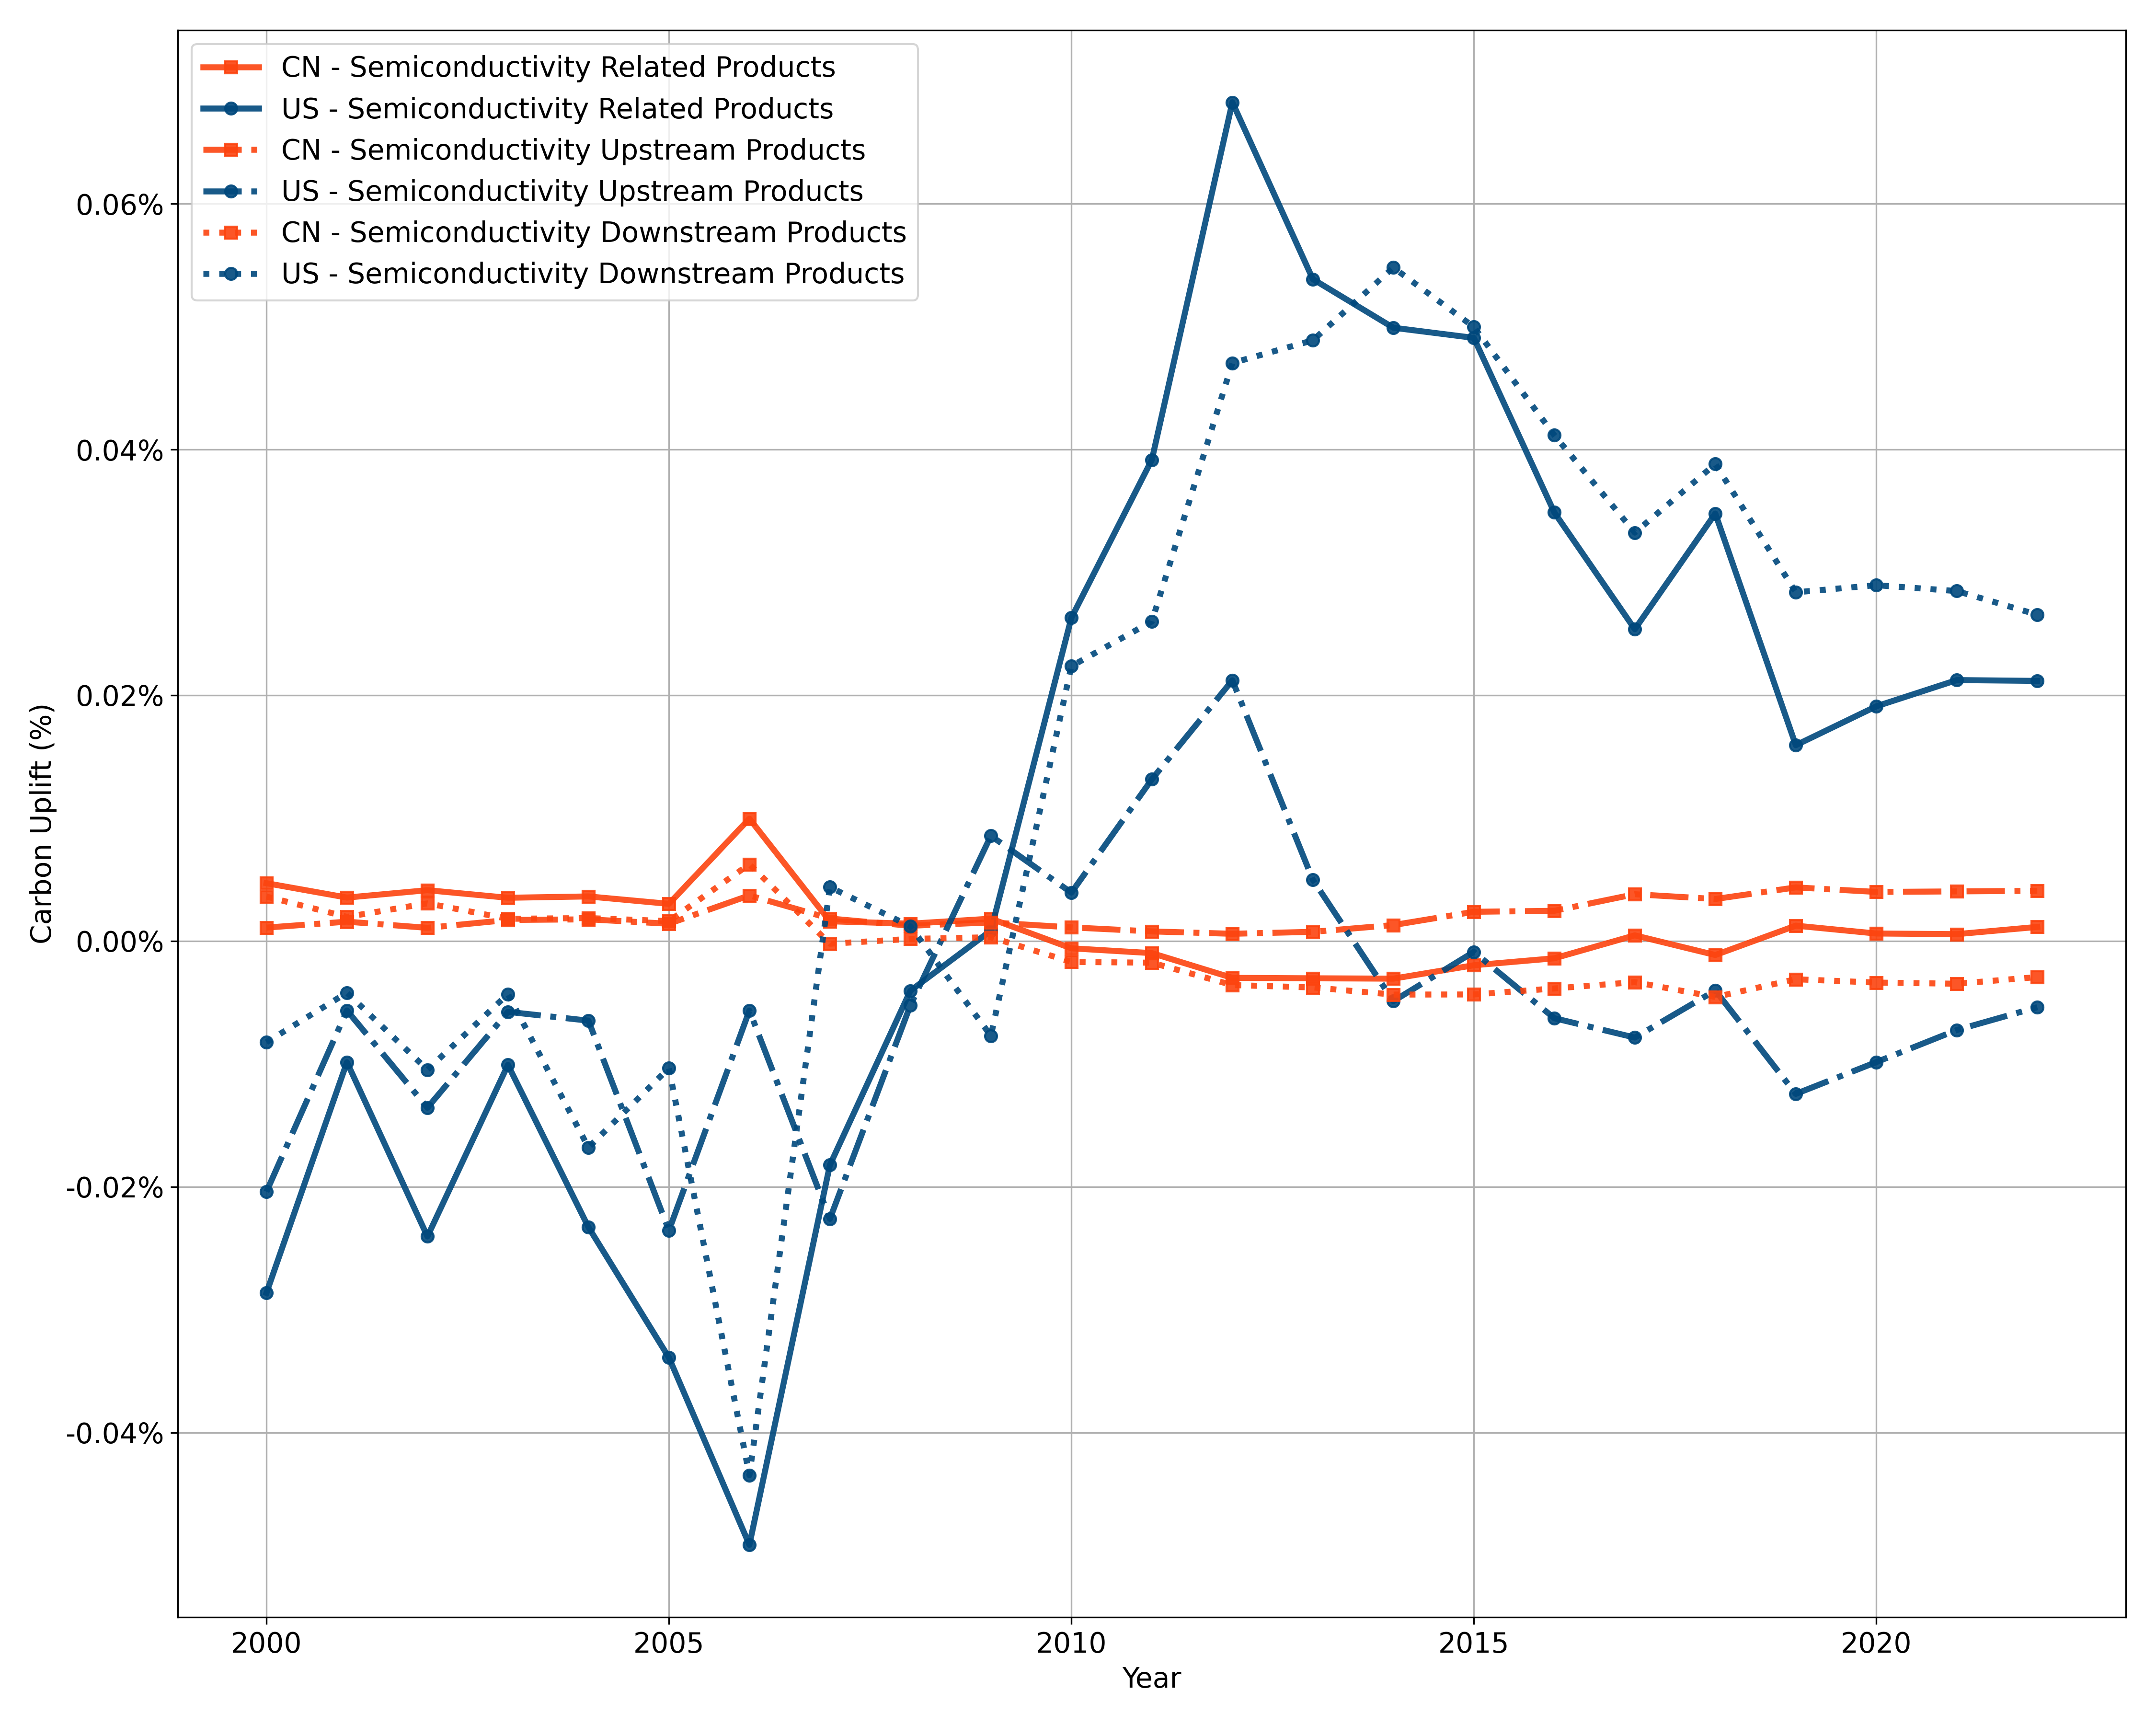
\includegraphics[width=1\textwidth]{figures/Graph/Carbon Uplift Trends If No Sino-US Trade(2000-2022).png}}
 \caption{Carbon Uplift Trends If No Sino-US Trade(2000-2022)}\label{fig:Carbon Uplift Trends If No Sino-US Trade(2000-2022)}
\end{figure}
\fi
\subsection{Carbon Uplift in No Sino-US Semi-conductor Related Products Trade with Gaming Scenario}

The analysis of carbon uplift in three distinct trade scenarios in 2022—absence of all trade, absence of Sino-U.S. trade, and a game theory-based reallocation of trade following a Sino-U.S. trade halt—reveals nuanced effects on carbon emissions on a global scale and across key nations, namely China and the United States, as shown in Figure \ref{fig:Comparison of Carbon Uplift between 3 Scenario}.

In the global context, the elimination of all trade induces a carbon uplift of 0.9106\% for semiconductivity-related products, indicating an increased global carbon footprint due to the localization of production. When bilateral trade between China and the U.S. ceases, the uplift is marginal at 0.0031\%, suggesting that while significant, the carbon footprint impact is not as substantial as one might presume given the volume of trade between these two economies.

The third scenario presents a game-theoretical distribution of trade voids left by halted Sino-U.S. trade, adjusted according to existing production structures and the proportional value output within industry supply chains. Here, a notable shift occurs: the global carbon uplift for related products pivots to 0.3568\%, a figure more pronounced than the no bilateral trade scenario but still less than the no trade scenario. This shift can be attributed to the strategic redistribution of production to regions that may not match the carbon efficiency of the previous Sino-U.S. configuration.

China's unique position as both a massive producer and consumer plays a pivotal role in these scenarios. Under game-theoretic reallocation, China experiences an increase in carbon uplift for related products to 1.2301\%, suggesting that the reallocation may lead to less carbon-efficient production processes taking over the supply void. Conversely, the U.S. sees an uplift of 0.7731\% for related products, hinting at potential increases in carbon emissions due to adjusted trade patterns and possibly less efficient domestic production filling the gap.
\ifincludefigures
\begin{figure}
  \centering
  \makebox[\textwidth][c]{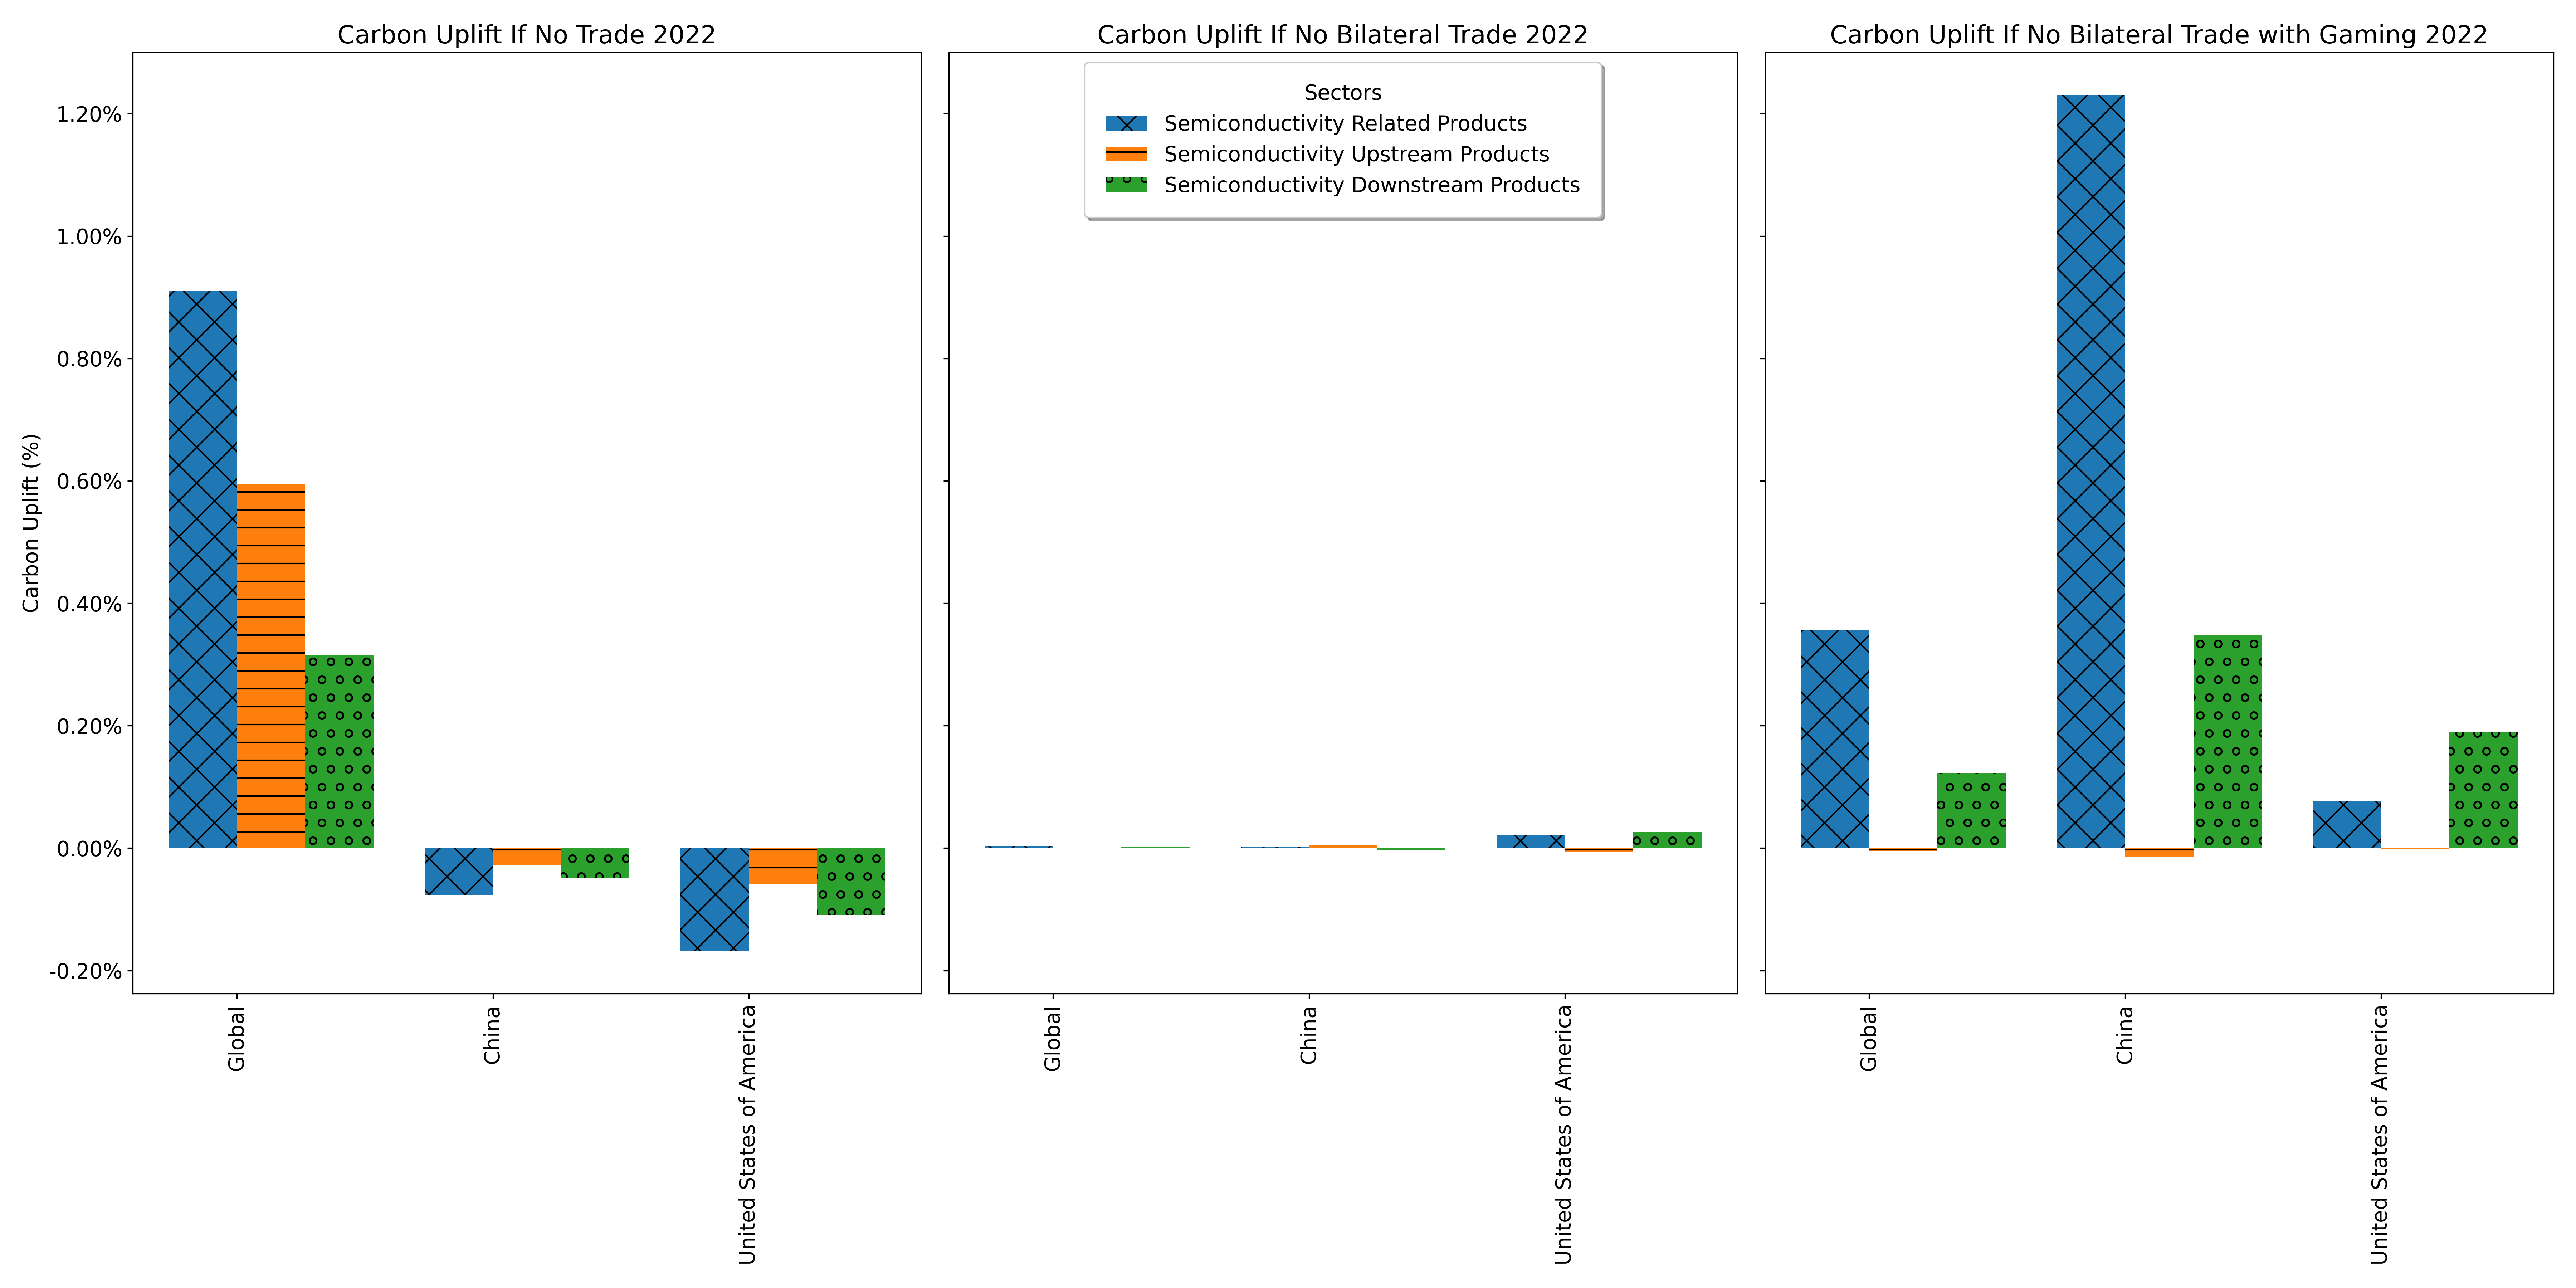
\includegraphics[width=1\textwidth]{figures/Graph/Comparison of Carbon Uplift between 3 Scenario.png}}
  \caption{Comparison of Carbon Uplift between 3 Scenario}\label{fig:Comparison of Carbon Uplift between 3 Scenario}
 \end{figure}
\fi
 In the scenario framed by game theory distribution Figure \ref{fig:Carbon Uplift Trends If No Sino-US with Gaming Trade(2000-2022)}, the strategic reallocation of trade shares between the United States and China shows an upward trajectory in carbon uplift over the years. This model, which diverges from a simplified binary trade or no-trade paradigm Figure \ref{fig:Carbon Uplift Trends If No Sino-US Trade(2000-2022)}, suggests a more complex interaction within the global supply chain, where the interdependence of international trade plays a crucial role.

 The analysis reveals that the carbon uplift in the gaming scenario substantially exceeds the uplift in the simple scenario of domestic production replacing imports. This outcome challenges the notion that ceasing Sino-US trade would lead to a straightforward transition to domestic production for either country. Moreover, the fact that the uplifts are more pronounced under the gaming scenario may imply that the simplified scenario fails to capture the dynamic efficiencies and the clean production structures already present in the Chinese and American industries, which are among the most carbon-efficient on the global stage.
 
 A closer look at the data from 2000 to 2022 reflects this trend. For instance, in the year 2022, China's carbon uplift for semiconductor-related products under the gaming scenario was 1.2301\%, marking a stark contrast to a more modest uplift in the no-trade scenario. Similarly, the United States also exhibited an uplift in the gaming scenario, with figures like 0.7731\% for the year 2022 for semiconductor downstream products. These specific numbers indicate that the advantages of trade in carbon efficiency are not fully realized when trade is simply redistributed without considering the underlying economic and environmental efficiencies.
 
 The larger carbon uplifts observed in this game theory-informed scenario suggest that a hypothetical redistribution of trade shares may lead to less optimal environmental outcomes than the current state of trade. It underscores the potential misalignment between economic strategies and environmental goals, highlighting the importance of considering the full spectrum of supply chain dynamics when assessing the environmental impacts of trade policies.
 \ifincludefigures
 \begin{figure}
  \centering
  \makebox[\textwidth][c]{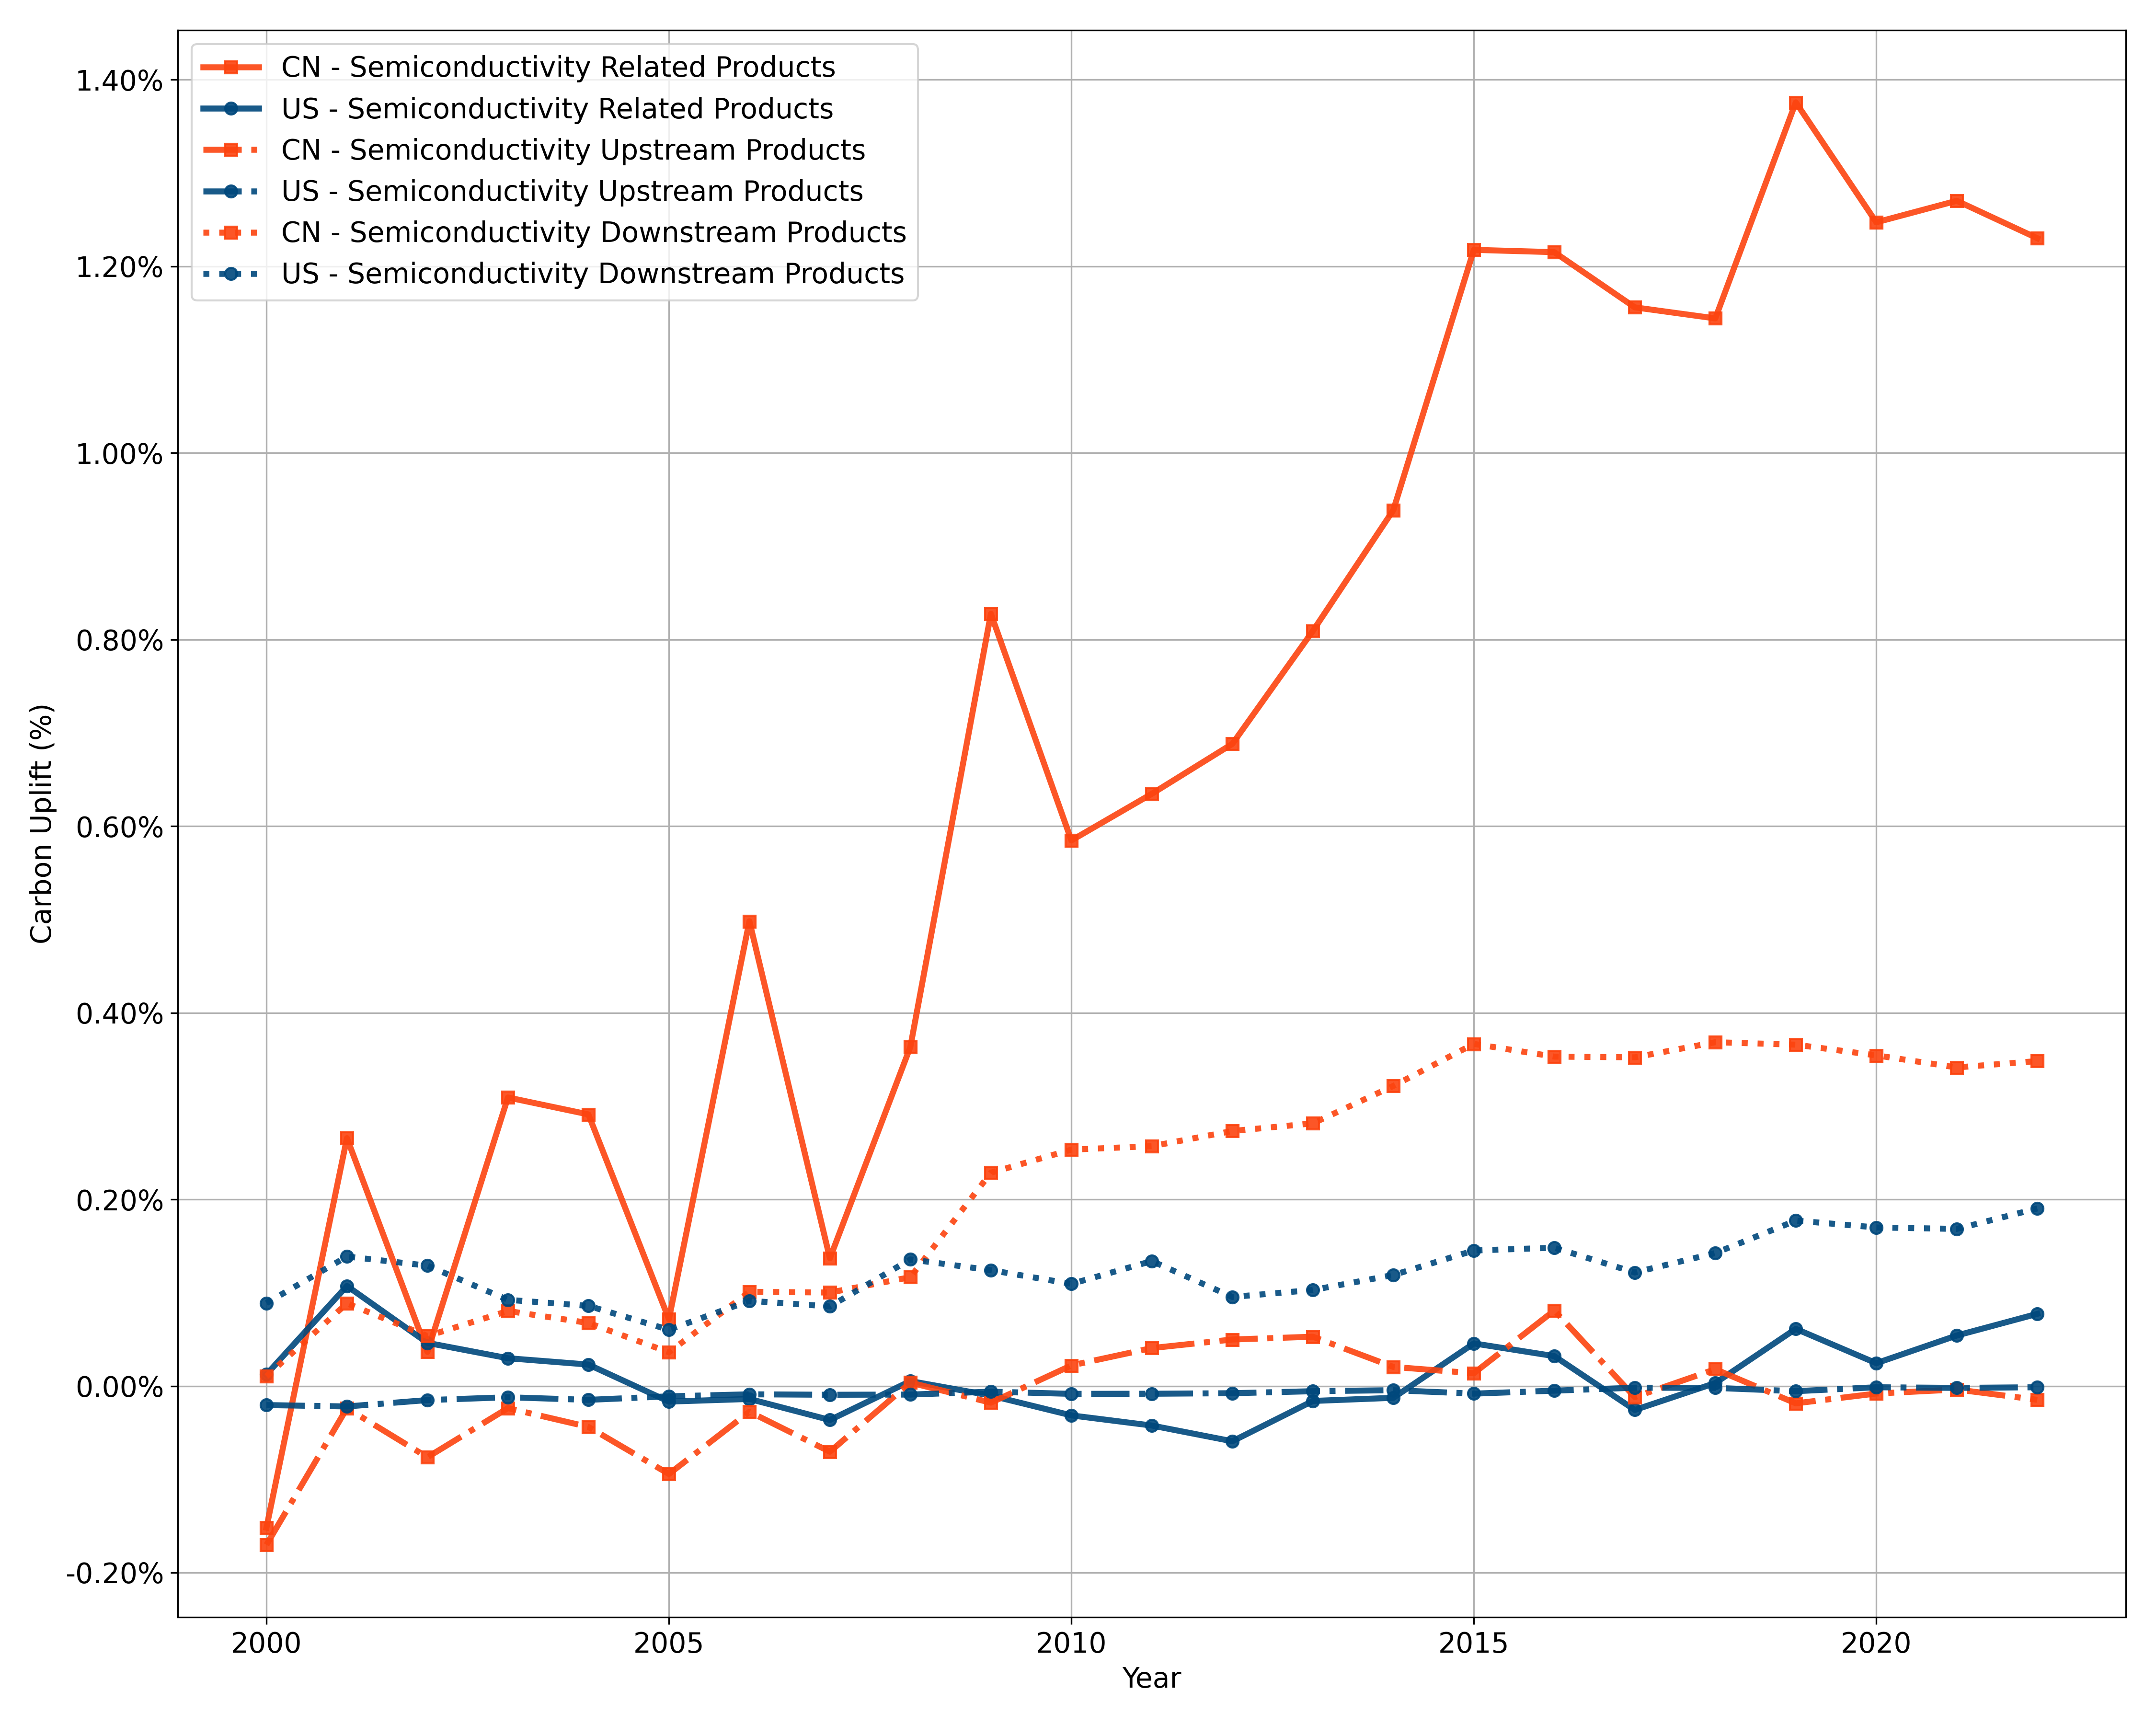
\includegraphics[width=1\textwidth]{figures/Graph/Carbon Uplift Trends If No Sino-US with Gaming Trade(2000-2022).png}}
  \caption{Carbon Uplift Trends If No Sino-US with Gaming Trade(2000-2022)}\label{fig:Carbon Uplift Trends If No Sino-US with Gaming Trade(2000-2022)}
 \end{figure}
\fi
% \subsection{Net Semi-Conductor Export Ratio vs. Carbon Uplift If No Sino-US Trade with Gaming}

% \begin{figure}
%   \centering
%   \makebox[\textwidth][c]{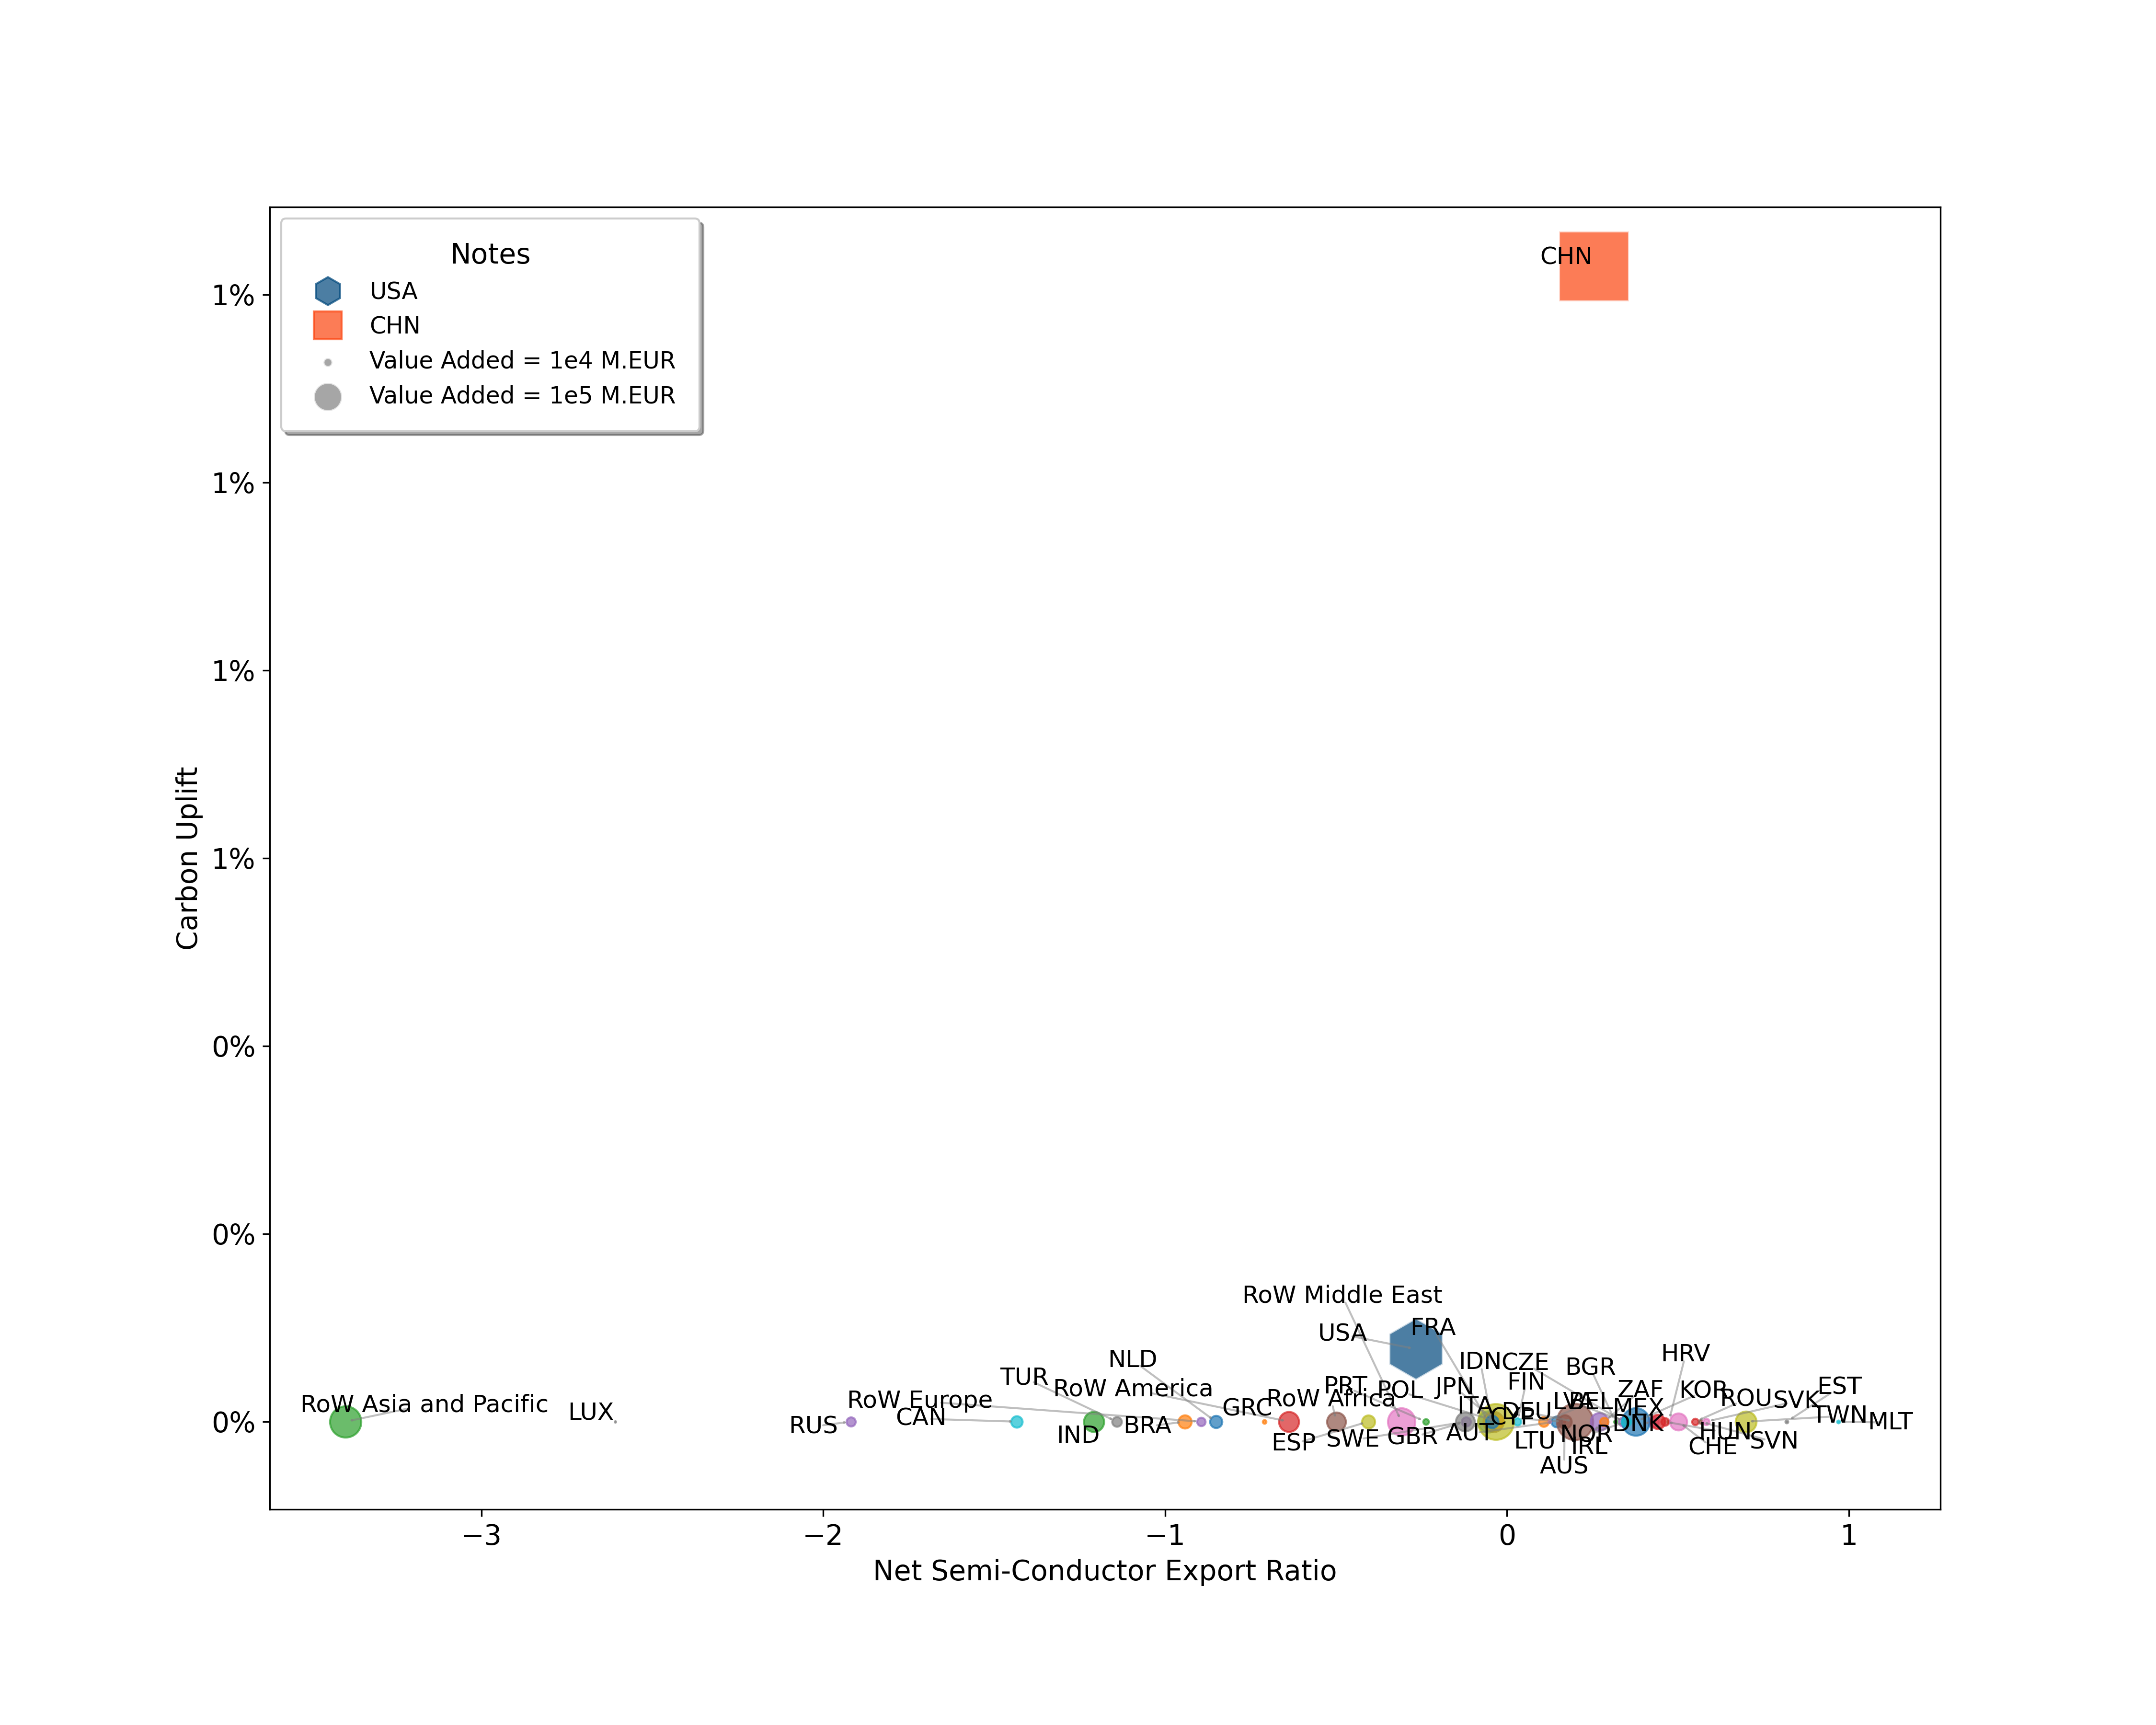
\includegraphics[width=1\textwidth]{figures/Graph/Net Semi-Conductor Export Ratio vs. Carbon Uplift If No Sino-US Trade with Gaming.png}}
%   \caption{Net Semi-Conductor Export Ratio vs. Carbon Uplift If No Sino-US Trade with Gaming}\label{fig:Net Semi-Conductor Export Ratio vs. Carbon Uplift If No Sino-US Trade with Gaming}
%  \end{figure}


\section{Comparison of Global Carbon Stressors}
\subsection{Rank of Carbon Stressors in 2022}
In the scholarly discourse examining the semiconductor industry's carbon footprint, we center upon the segmentation of upstream and downstream sectors. Figure \ref{fig:Rank of Carbon Stressor Heatmap in 2022} provides a granular perspective on the environmental costs of semiconductor production.

For the upstream segments, ``Other non-ferrous metal ores and concentrates'' denote significant carbon stressors, with China presenting approximately 221,397 kg CO2 per M EUR, juxtaposed against the United States`` higher output of around 360,391 kg CO2 per M EUR. In the arena of ''Precious metals" another upstream category, China again indicates a robust emission figure of roughly 304,336 kg CO2 per M EUR, while the United States showcases a lower, yet substantial, figure of approximately 75,648 kg CO2 per M EUR.

Transitioning to the downstream analysis, we observe in the sector ``Electrical machinery and apparatus n.e.c. (31)'' China's carbon stressor is noted at about 10,232 kg CO2 per M EUR, in contrast to the United States' figure of around 18,798 kg CO2 per M EUR. In the domain of ``Office machinery and computers (30)'' the carbon emission intensity for China is captured at nearly 9,244 kg CO2 per M EUR, with the United States reflecting a higher emission intensity of approximately 18,205 kg CO2 per M EUR. Moreover, within ``Radio, television and communication equipment and apparatus (32)'' China's carbon stressor stands at around 25,205 kg CO2 per M EUR, with the United States slightly elevated at 22,833 kg CO2 per M EUR. Lastly, in the ``Medical, precision and optical instruments, watches and clocks (33)'' sector, the data delineate China at roughly 5,285 kg CO2 per M EUR and the United States at about 22,749 kg CO2 per M EUR.

The visualization method adopted in the paper, the ``Rank of Carbon Stressor Heatmap in 2022'' is predicated upon a ranking-based depiction rather than raw numerical values. This analytical choice is made to circumvent the limitations posed by the disparate magnitude of raw data, ensuring a more coherent and comparative visual comprehension of the carbon stressors across various sectors and countries.
\ifincludefigures 
\begin{figure}
 \centering
 \makebox[\textwidth][c]{\includegraphics[width=1\textwidth]{figures/Graph/Rank of Carbon Stressor Heatmap in 2022.png}}
 \caption{Rank of Carbon Stressors Heat Map in 2022}\label{fig:Rank of Carbon Stressor Heatmap in 2022}
\end{figure}
\fi
\subsection{Carbon Stressor Trends (2000-2022)}
The intricate graph Figure \ref{fig:Carbon Stressor Trends (2000-2022)} delineates the carbon stressor in kilograms of CO2 equivalent per million EUR of product value (kg CO2 eq./M EUR) for China, the United States, and globally, across all products and within the semiconductor sector, including both its upstream and downstream components.

Beginning the analysis with the year 2000, China's carbon stressor in the semiconductor industry's related products was 140,031 kg CO2 eq./M EUR, which, when compared to the upstream and downstream sectors—1,466,154 and 63,334 kg CO2 eq./M EUR, respectively—indicates a significant carbon efficiency in the production of specific semiconductor-related outputs. Over the subsequent years, a downward trend is evident, with fluctuations that suggest adjustments and improvements in production efficiency, concluding with the 2022 figures of 24,511 kg CO2 eq./M EUR for related products, and 141,159 kg CO2 eq./M EUR for downstream, against an upstream value of 271,619 kg CO2 eq./M EUR.

For the United States, the year 2000 starts with a carbon stressor of 433,602 kg CO2 eq./M EUR for related products, and 372,360 and 405,985 kg CO2 eq./M EUR for the downstream and upstream sectors, respectively. This highlights a greater initial carbon stressor compared to China. Over the years, the US shows a trend of reducing this stressor across all sectors, particularly in the related and downstream products, culminating in 2022 with values of 22,343 and 21,392 kg CO2 eq./M EUR for related and downstream products, and a higher but reduced upstream stressor of 83,254 kg CO2 eq./M EUR.

The global trends mirror this reduction, starting from 71,282 kg CO2 eq./M EUR for related products and 53,260 and 658,171 kg CO2 eq./M EUR for downstream and upstream sectors in 2000, to 46,830 and 35,374 kg CO2 eq./M EUR for related and downstream products, and 344,678 kg CO2 eq./M EUR for upstream products in 2022. The general trend shows a global drive towards higher carbon efficiency, albeit with regional disparities.

The relationship between these carbon stressors and the previously discussed carbon uplift in a no-trade scenario is telling. The carbon stressor is a measure of the efficiency of production—a lower figure suggests a higher carbon efficiency. In the absence of trade, especially between China and the US, we see the carbon uplift—representing an increase in carbon emissions—reducing over time, which could imply that the efficiency of local production is increasing, thus lessening the potential negative environmental impacts of trade disruptions. This supports the initial analysis that suggests that the semiconductor industry, particularly in China and the US, is advancing towards greater carbon efficiency. Despite this progress, the complexities of global trade and production processes indicate that continuous improvements and collaborations are necessary to further mitigate the carbon footprint of this vital sector.
\ifincludefigures
\begin{figure}
 \centering
 \makebox[\textwidth][c]{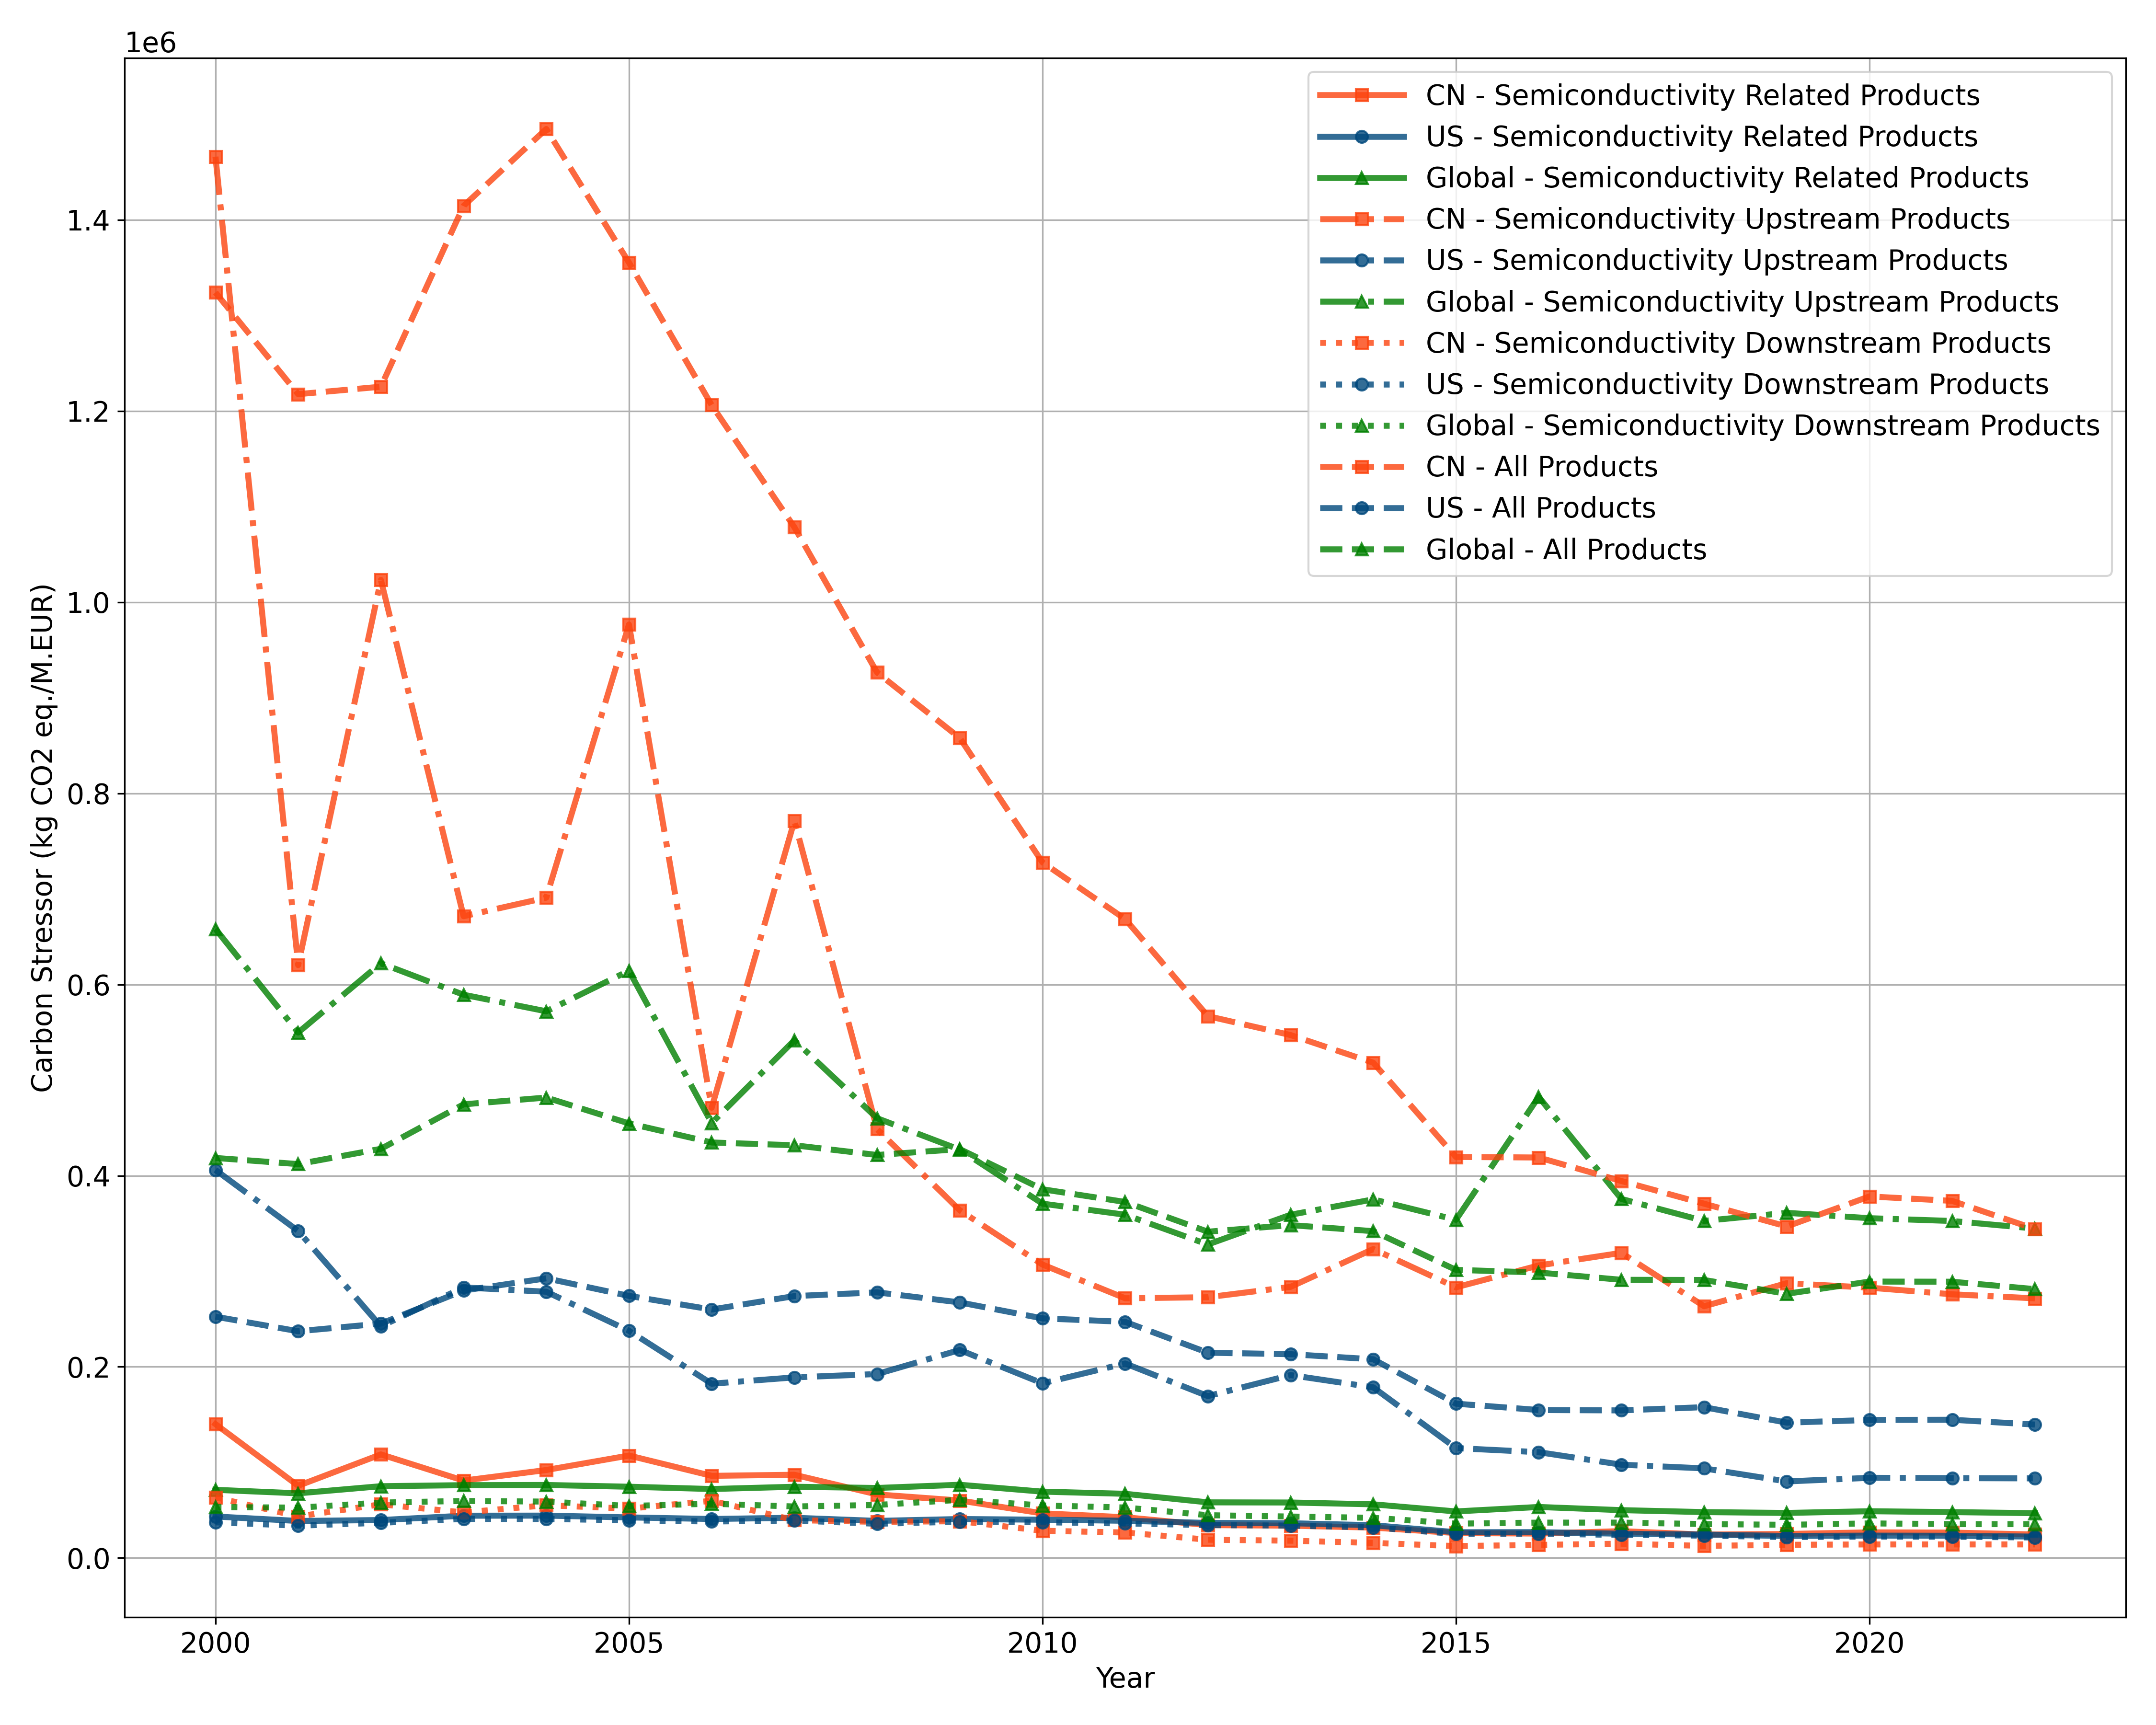
\includegraphics[width=1\textwidth]{figures/Graph/Carbon Stressor Trends (2000-2022).png}}
 \caption{Carbon Stressors Trends (2000-2022)}\label{fig:Carbon Stressor Trends (2000-2022)}
\end{figure}
\fi
\subsection{Carbon Stressor in Different Sectors 2022}
Figure \ref{fig:Carbon Stressor in Different Sectors 2022} reveals the heterogeneous nature of the carbon stressor across regions and sectors, underscoring the complex interdependencies and varied stages of development. The metric, measured in kilograms of CO2 equivalent per product value, illuminates the environmental cost of economic activities. 

Africa's substantial carbon stressor figures (approx. 249,685 kg CO2 eq./M EUR for related products) hint at the potential for improvement in production efficiencies or the necessity for technology transfer to reduce the environmental impact of its burgeoning semiconductor industry.

Focusing on the Americas, the data depicts a relatively low carbon stressor in the related products sector at approximately 27,254 kg CO2 eq./M EUR, which, juxtaposed with the significant figure in the upstream sector (approx. 178,097 kg CO2 eq./M EUR), indicates a remarkable discrepancy between the different stages of semiconductor production.

China (CHN), a key player in this narrative, shows a carbon stressor of approximately 24,511 kg CO2 eq./M EUR for related products and 141,159 kg CO2 eq./M EUR for downstream products. These figures, when aligned with its upstream carbon stressor of about 271,619 kg CO2 eq./M EUR, suggest a more efficient downstream production relative to the upstream processes.

When we consider the United States (USA), the carbon stressor in related semiconductor products is approximately 22,343 kg CO2 eq./M EUR, with the upstream value at 83,254 kg CO2 eq./M EUR, and downstream at about 21,392 kg CO2 eq./M EUR. This denotes a more balanced carbon stressor across the sectors compared to other regions, reflecting perhaps a more mature market with optimized production processes.

The global view encapsulates these variances, with a general carbon stressor in semiconductor-related products at approximately 46,830 kg CO2 eq./M EUR, indicating the worldwide impact of this industry. This serves as a critical indicator for policymakers and industry leaders to assess and strategize for a sustainable progression of the semiconductor industry.
\ifincludefigures
\begin{figure}
 \centering
 \makebox[\textwidth][c]{\includegraphics[width=1\textwidth]{figures/Graph/Carbon Stressor in Different Sectors 2022.png}}
 \caption{Carbon Stressors in Different Sectors 2022}\label{fig:Carbon Stressor in Different Sectors 2022}
\end{figure}
\fi
